\documentclass[a4paper, 10pt]{article}
\usepackage{polski}
\usepackage[utf8]{inputenc}
\usepackage{amsmath}
\usepackage{graphicx}
\usepackage{caption}
\usepackage{subcaption}
\usepackage{geometry}
\usepackage{float}



\graphicspath{{./img/}}

\title{MGR - Raport 1}
\author{Jakub Postępski}

\begin{document}

\maketitle

\section{Problem}
Należy skompensować siłę grawitacji w układzie stawu obrotowego sterowanego impedancyjnie. Rozwiązaniem jest określenie masy a następnie dodanie odpowiednich sił do układu w celu kompensacji siły grawitacji.

\section{Obiekt}
Obiektem jest układ wahadła sterowanego prawem sterowania impedancyjnego (rys. \ref{fig:2d}). Na końcu nieważkiego ramienia $r$ zawieszona jest punktowa masa $m$ której grawitację należy skompensować. Algorytm sterowania symuluje sprężynę oraz amortyzator w osi obrotu wahadła i można do niego dodać moment $u$. W osi obrotu znajduje się czujnik FTS. Przyjmujemy że dla użytkownika dostępne są pomiary położenia $q$, prędkości $\dot{q}$, przyspieszenia $\ddot{q}$ oraz pomiary siły $F$ i momentu siły $\tau$.

Układ z inercją $I$ możemy opisać przy pomocy równania:
\begin{equation}
\label{eq:intro}
\tau = I\ddot{q} = mr^2\ddot{q} = kq + d\dot{q} + mg\cos{(q)} + Iu
\end{equation}

Model obiektu można opisać układem równań różniczkowych:
\begin{equation}
	\begin{bmatrix}
	    \dot{q} \\
	    \ddot{q}
	\end{bmatrix}
	=
	\begin{bmatrix}
	    0 & 1 \\
	    \frac{k}{I} & \frac{d}{I}
	\end{bmatrix}
	\begin{bmatrix}
		q \\
	    \dot{q}
	\end{bmatrix}
	+
	\begin{bmatrix}
	    0 \\
	    1
	\end{bmatrix}
	(\frac{mg\cos{(q)}}{I} + u)
\end{equation}

gdzie:
\begin{itemize}
	\item $q$ - kąt obrotu [$rad$]
	\item $k$ - sztywność
	\item $b$ - tłumienie
	\item $m$ - masa przedmiotu [$kg$]
	\item $g$ - przyspieszenie ziemskie [$\frac{m}{s^2}$]
	\item $u$ - moment który można zewnętrznie dodać do układu [$Nm$]
\end{itemize}

Układ możemy więc zapisać w standardowej postaci
\begin{equation}
\dot{q} = \textbf{A}q + \textbf{B}u(t)
\end{equation}
gdzie:
\begin{equation}
\mathbf{A} = 	\begin{bmatrix}
	    0 & 1 \\
	    \frac{k}{I} & \frac{d}{I}
	\end{bmatrix}
\end{equation}
oraz:
\begin{equation}
\mathbf{B} = \begin{bmatrix}
	    0 \\
	    1
	\end{bmatrix}
\end{equation}

Siła działająca na układ jest sumą siły grawitacji i siły odśrodkowej układu.
Siłę grawitacji możemy opisać wzorem:
\begin{equation}
F_g = mg
\end{equation}
a siłę odśrodkową odpowiednio w osi $X$ oraz $Y$ wzorami:
\begin{equation}
F_{ox} =  \cos{m(\dot{q}^2 r)}
\end{equation}
\begin{equation}
F_{oy} =  \sin{m(\dot{q}^2 r)}
\end{equation}


Dlatego odczyty czujnika w dwóch osiach możemy opisać wzorami:
\begin{equation}
F_y = F_g + F_{oy} = mg + \sin{m(\dot{q}^2 r)}
\end{equation}
\begin{equation}
F_x = F_{ox} = m\cos{m(\dot{q}^2 r)}
\end{equation}

\section{Dyskretyzacja układu}
Po zdyskretyzowaniu metodami ZOH z okresem próbkowania $T$ otrzymujemy układ:
\begin{equation}
q(t+1) = \mathbf{A_d}q(t) + \mathbf{B}_du(t)
\label{eq:dyskretny}
\end{equation}

Dyskretyzację odczytów FTS można przeprowadzić korzystając z równań zdyskretyzowanych metodą Eulera ($\dot{q} \approx \frac{q(t)-q(t-1)}{T}$). 

\begin{equation}
F_x(t) = m\cos{((\frac{q(t)-q(t-1)}{T})^2 r)}
\end{equation}
\begin{equation}
\label{eq:fy}
F_y(t) = mg + m\sin{((\frac{q(t)-q(t-1)}{T})^2 r)}
\end{equation}

oraz z równania \ref{eq:intro}
\begin{equation}
\tau(t) = kq(t) + d\frac{q(t)-q(t-1)}{T} + Iu + mg\cos(q)
\end{equation}

Podobnie można dyskretyzować inne równania.
\section{Estymacja nieznanych parametrów}
W celu skompensowania grawitacji zawieszonej masy należy poznać parametry opisujące tę masę. Uznano że do opisu wystarczą typowe i powszechnie używane zmienne. W opisywanym układzie nie są znane takie wielkości jak inercja, masa oraz środek ciężkości. 

Przy założeniu, że masa jest punktowa wiemy że inercję tej masy opisuje zależność
\begin{equation}
I = mr^2
\end{equation}
W trakcie opisu metod estymacji parametrów starano się w miarę możliwości nie korzystać z tej zależności. Dzięki takiemu podejściu w przyszłości będzie można wykorzystać znalezione metody w celu estymacji mas niepunktowych o nierównomiernym rozkładzie. 

Posiadając estymację promienia $r$ i wykorzystując pozycję $q$ jesteśmy w wstanie określić pozycję zawieszonej masy a więc i środek ciężkości.


\subsection{Estymacja masy z FTS, podejście naiwne}
\label{fts:nai}
Analizując składowe mierzone w osi $Y$ czujnika siły można wyodrębnić siłę grawitacji i utożsamić ją ze składową stałą sygnału. Kiedy zawieszona masa się nie porusza w łatwy sposób można odczytać siłę grawitacji. W momencie ruchu układu z czujnika dostajemy sygnał zmienny. W celu uzyskania składowej stałej (siły grawitacji) możemy zastosować transformatę Fouriera. W praktyce sygnał nie jest poddawany pełnej transformacji a do wyliczania składowej stałej syganłu użyty został filtr średniej kroczącej. Dodatkową zaletą zastosowania filtru jest niwelowanie szumów pomiarowych.

\subsection{Estymacja inercji z macierzy układu}
\label{sec:pos}
Ponieważ macierz $\mathbf{B}$ ma tylko jeden wyraz różny od zera $\mathbf{B_d}$ jest uzyskiwana w prosty sposób i można przyjąć że:
\begin{equation}
\mathbf{B_d} \approx \mathbf{B}T
\end{equation}
Przekształcając równanie \ref{eq:dyskretny} i stosując pseudoinwersję macierzy otrzymujemy równanie macierzowe:
\begin{equation}
\mathbf{A_d} = (X(t+1) - \mathbf{B}_du(t))(X(t))^{pinv}
\label{eq:pinv}
\end{equation}
przy założeniu $n$ ostatnich próbek zmiennych stanów układu
\begin{equation}
X(t) = 	\begin{bmatrix}
x(t) & x(t-1)  & ... & x(t-n)
\end{bmatrix}
\label{eq:xk}
\end{equation}

Po obliczeniu estymacji $\mathbf{A_d}$ metodą ZOH wyliczamy estymację macierzy $\mathbf{A}$ otrzymując macierz
\begin{equation}
\mathbf{\hat{A}} = 	\begin{bmatrix}
a_{11} & a_{12}\\
a_{21} & a_{22}
\end{bmatrix}
\end{equation}
Po przyrównaniu jej do macierzy $\mathbf{A}$ możemy wyliczć inercję z równań:
\begin{equation}
\hat{I_1} = \frac{-k}{a_{21}}
\end{equation}
\begin{equation}
\hat{I_2} = \frac{-b}{a_{22}}
\end{equation}

i ostatecznie przyjąć estymację:
\begin{equation}
\hat{I} = \frac{\hat{I_1}+\hat{I_2}}{2}
\end{equation}


\subsection{Estymacja masy przy wykorzystaniu FTS i wyliczeniu siły odśrodkowej}
\label{sec:ftsods}
Korzystając z równania \ref{eq:fy} można opisać siły działające na czujnik w osi $Y$ w chwili $i$ jako:
\begin{equation}
F_{yi}  = m(g + \dot{q_i}^2r\sin{(q_i)})
\end{equation}

Zakładając błędy odczytu $e$ dostajemy próbkę postaci:
\begin{equation}
\hat{F_{yi}}+e_i  = F_{yi}
\end{equation}

Posiadając $n$ próbek możemy więc sformuować zadanie optymalizacji nieliniowej z parametrami $m$ oraz $r$ takie że:
\begin{equation}
\begin{aligned}
& \underset{m, r}{\text{min}}
& & \sum_{i = 1}^{n} || e_i || = \sum_{i = 1}^{n} || \hat{F_{yi}} - F_{yi} || \\
& \text{przy ograniczeniach}
& & F_{yi} = m(g + \dot{q_i}^2r\sin{(q_i)}), \; i = 1, \ldots, n.
\end{aligned}
\end{equation}

Zadany problem optymalizacji nieliniowej można rozwiązać algorytmem Levenberga–Marquardta i ten algorytm jest wykorzystywany w badaniach.


\subsection{Estymacja masy przy wykorzystaniu równań na podstawie inercji}
Korzystajać z równania \ref{eq:intro} i znając inercję jesteśmy w stanie wyliczyć masę:
\begin{equation}
m = \frac{I\ddot{q} - kq - d\dot{q} -Iu}{g\cos{(q)}}
\end{equation}

Zastosowania równania w układzie z czasem dyskretnym zastosowano emulacje metodą Eulera i uzyskano:
\begin{equation}
m(t) \approx \frac{I\frac{q(t)-2q(t-1)+q(t-2)}{T^2}-kq(t)-d\frac{q(t)-q(t-1)}{T}-Iu}{g\cos(q)}
\end{equation}

Wadą rozwiązania są dwie osobliwości dla $q = \frac{\pi}{2}$ oraz $q = 3\frac{\pi}{2}$

\section{Symulacja układu}

Symulację obiektu (rys. \ref{fig:system}) można wykonać korzystając z wersji dyskretnej układu. W celu symulacji zakłóceń w każdym kroku symulacji zmiennych stanu układu dodawany jest szum biały.

\begin{figure}[H]
	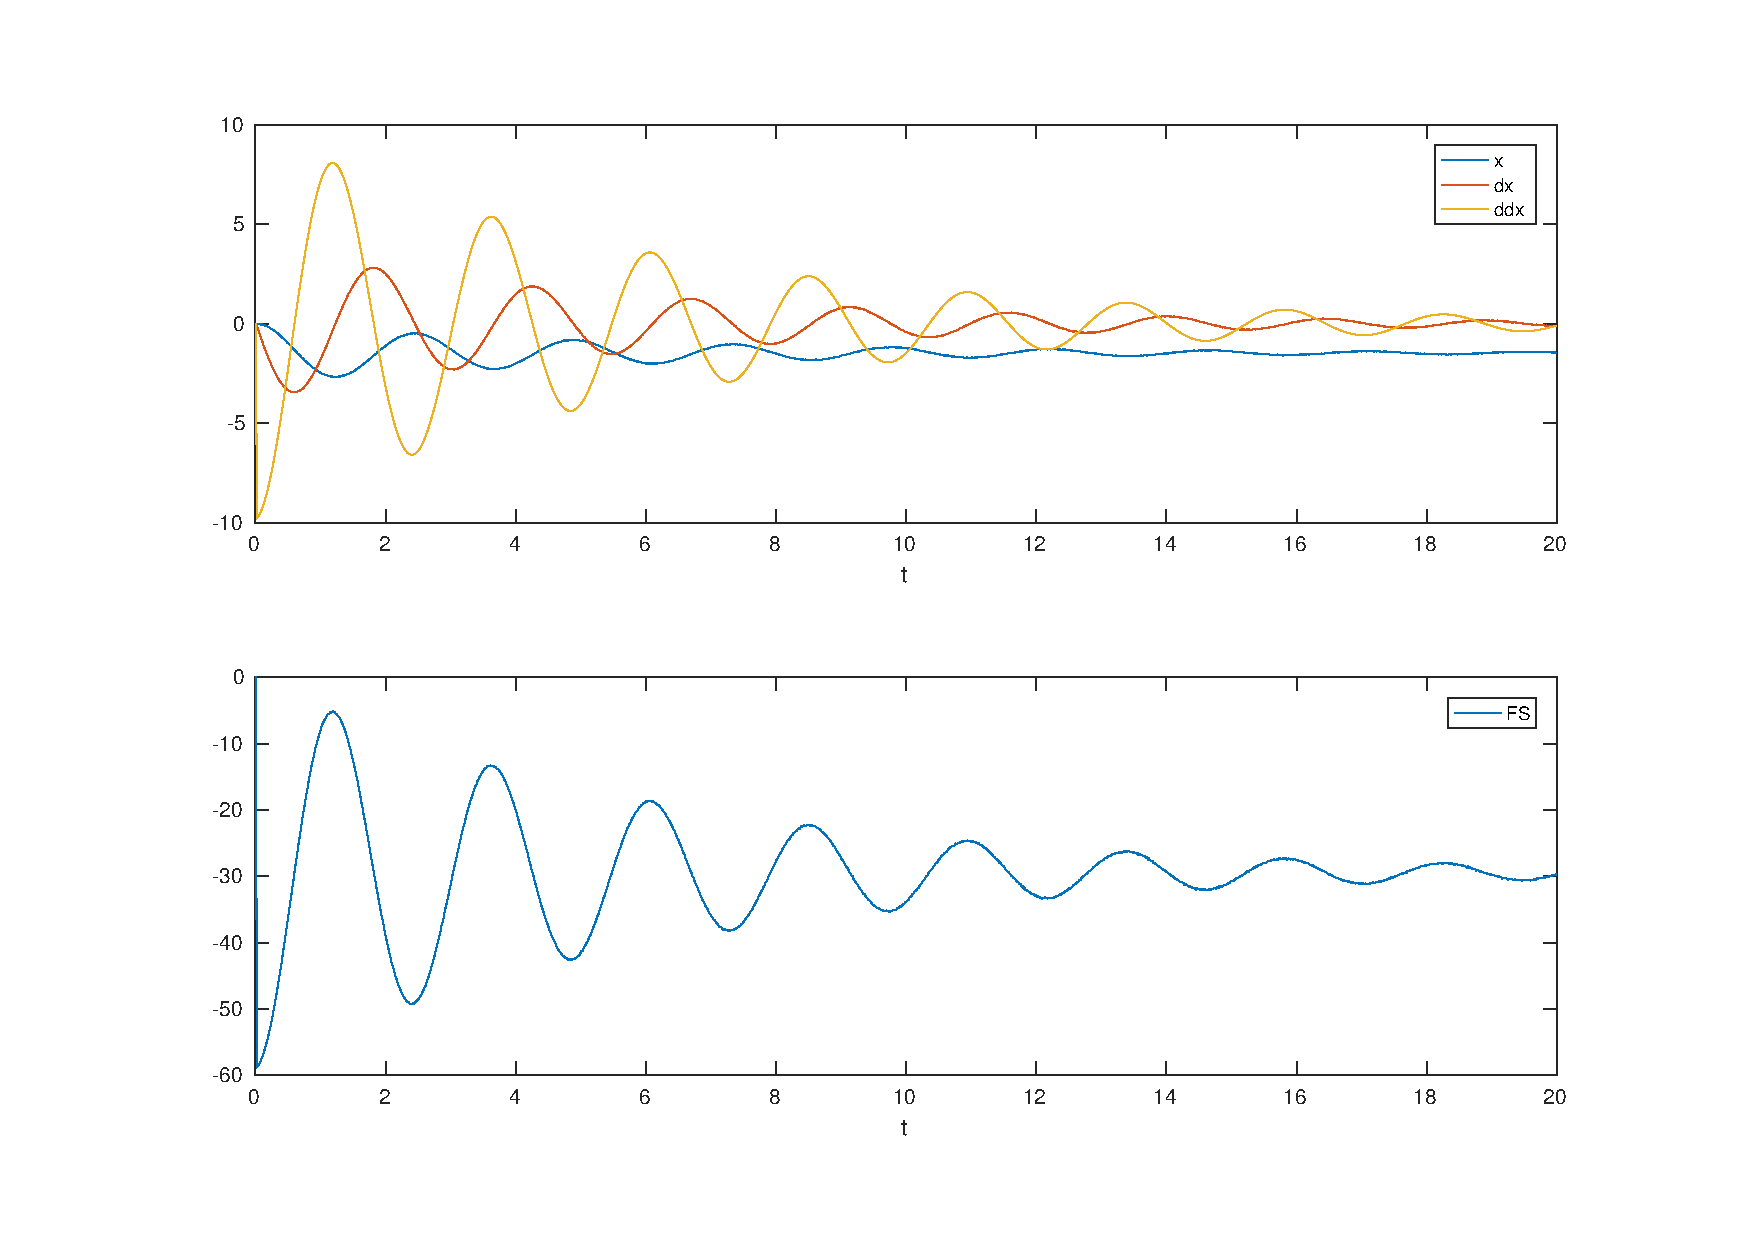
\includegraphics[width=0.99\linewidth]{system_sys}
	\centering
	\caption{Symulacja układu z parametrami $T=0.01$, $k = 20$, $b = 1$, $m = 3$.}
	\label{fig:system}
\end{figure}


\begin{figure}[H]
%	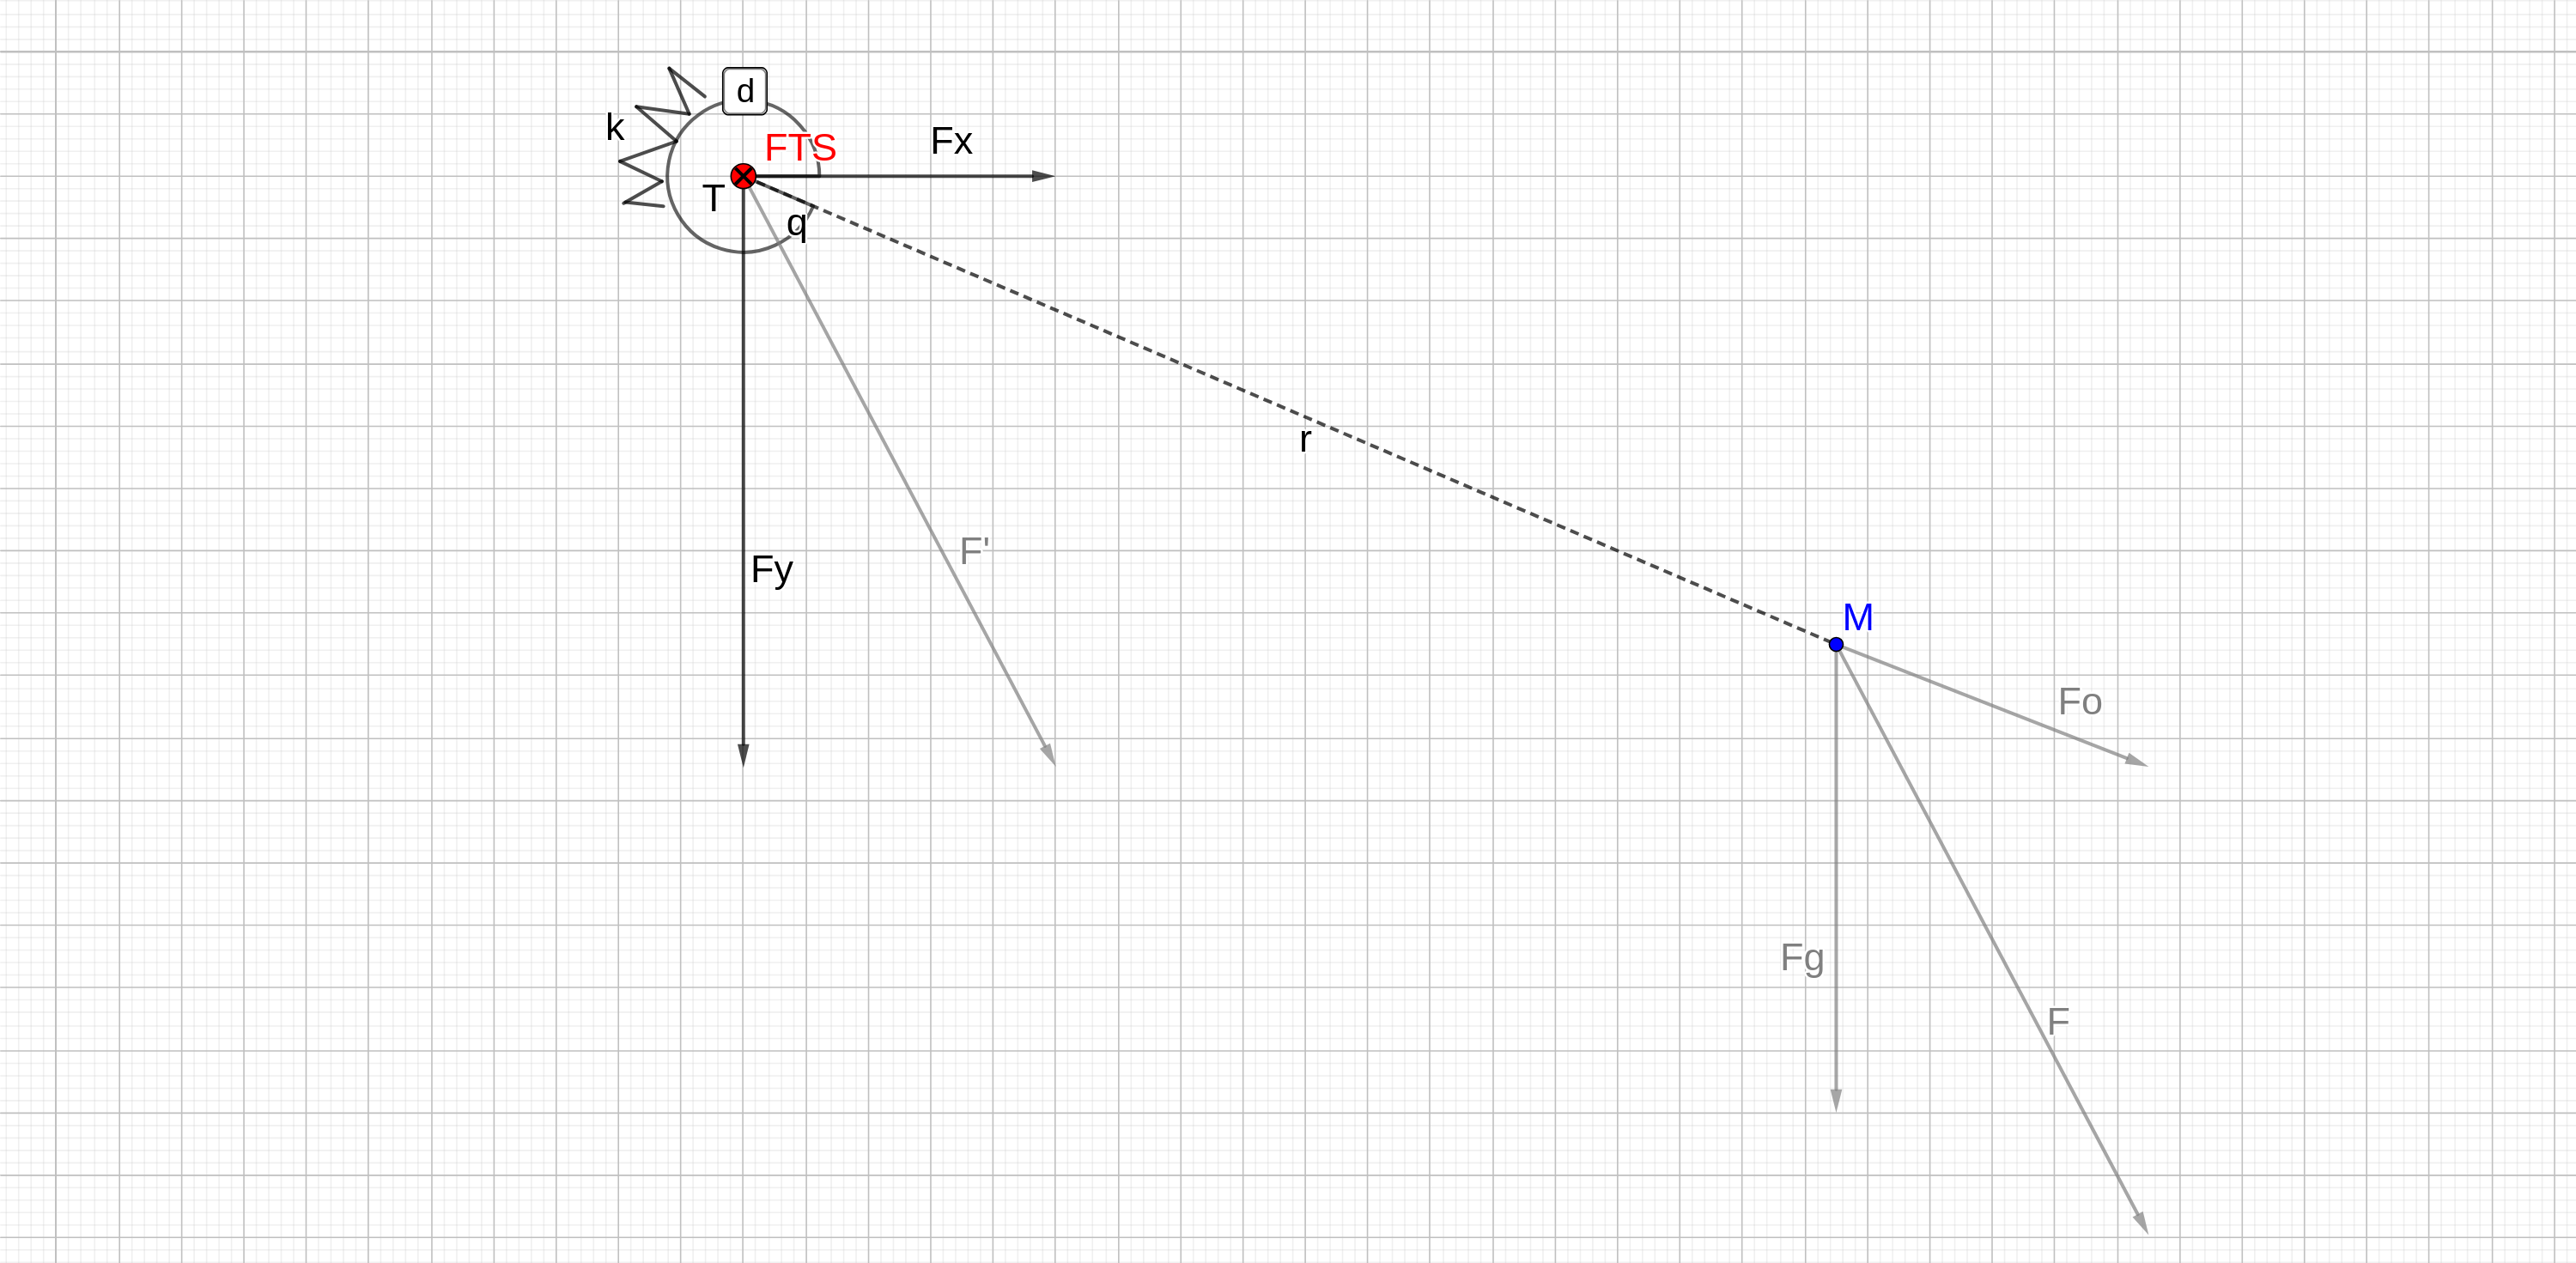
\includegraphics[width=0.99\linewidth]{2d}
	\centering
	\caption{Schemat badanego układu. Kolorem niebieskim zaznaczono masę $m$ zawieszoną na ramieniu $r$. Kolorem czerwonym zaznaczono punkt mocowania ramienie i umiejscowienia czujnika FTS. Kolorem czarnym pokazano siły odczytywane z czujnika sił, moment siły $\tau$, pozycję $q$ sprężynę $k$ oraz amortyzator $d$. Kolorem szarym zaznaczono rzeczywiste siły układu.}
	\label{fig:2d}
\end{figure}


\section{Symulacje}

W trakcie symulacji eksperymentalnie dobierano ilość próbek branych pod uwagę przez filtr. Dla filtrów z krótkim oknem (rys. \ref{fig:systemfs4_mass}, \ref{fig:systemfs100_mass}) widać, że są w stanie odfiltrować jedynie szumy pomiarowe czujnika. Dla filtrów z długim oknem widać, że potrzeba dużo czasu aby otrzymać estymację masy (rys. \ref{fig:systemfs1000_mass}). Finalnie wybrano okno długości $n = 500$ (rys. \ref{fig:systemfs500_mass}.)

\begin{figure}[H]
	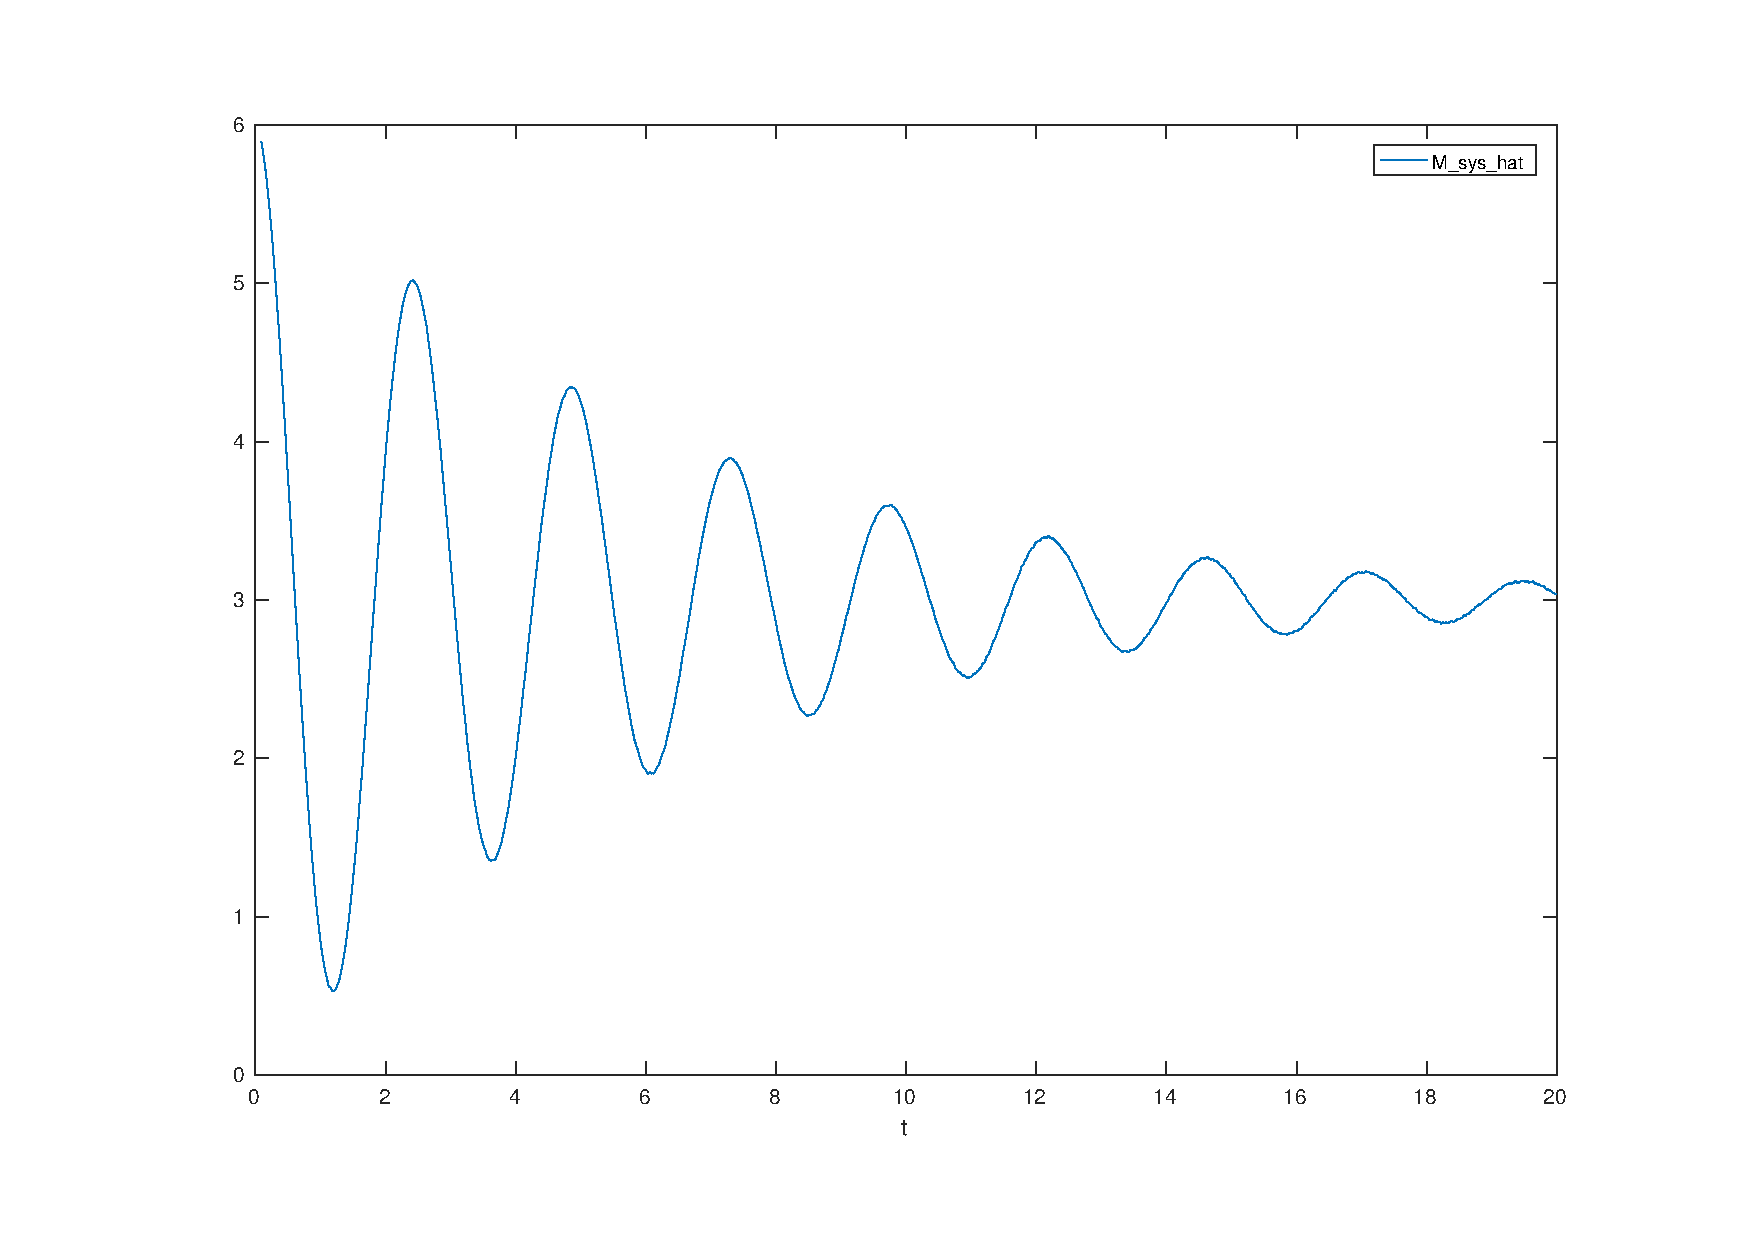
\includegraphics[width=0.99\linewidth]{systemfs4_mass}
	\centering
	\caption{Estymacja masy układu z parametrami $T=0.01$, $k = 20$, $b = 1$, $m = 3$ dla 4 próbek używanych w alogrytmie średniej kroczącej. }
	\label{fig:systemfs4_mass}
\end{figure}

\begin{figure}[H]
	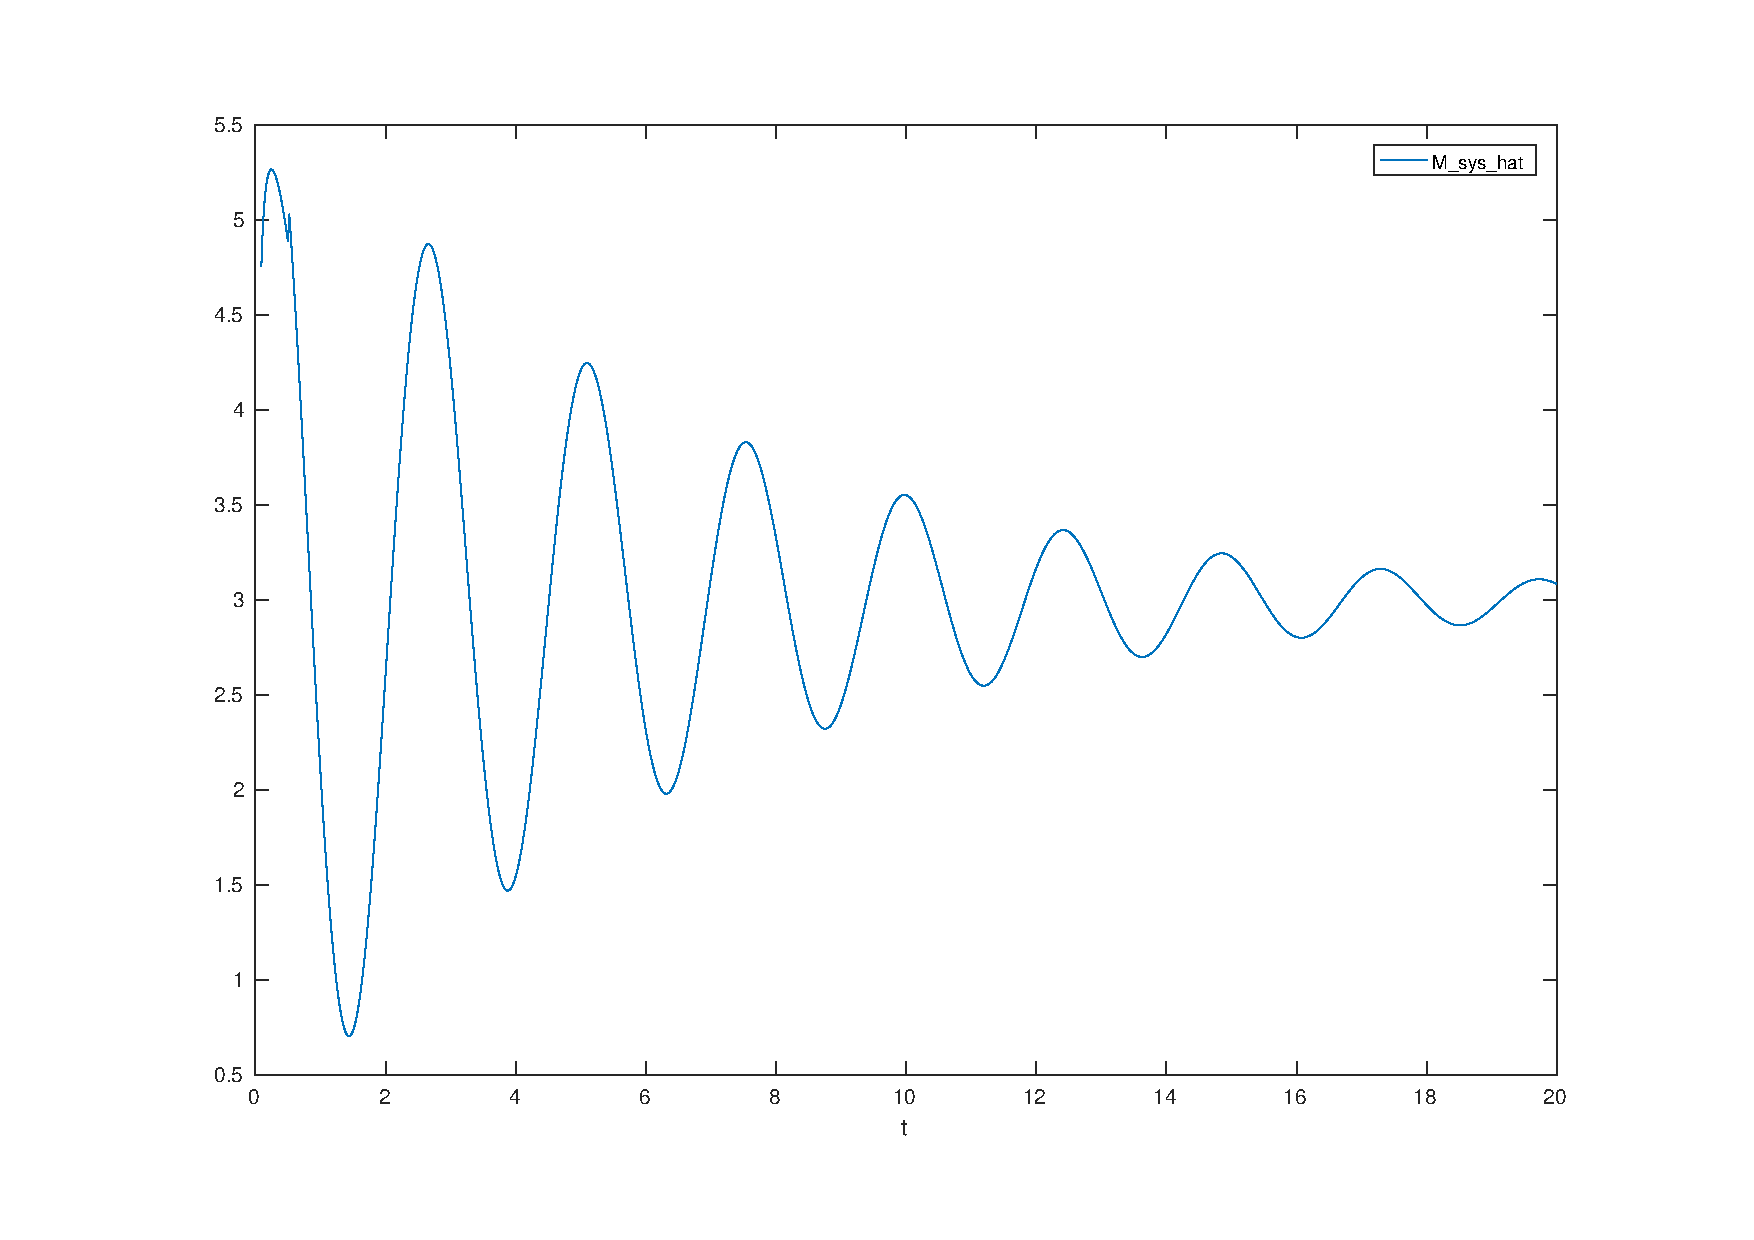
\includegraphics[width=0.99\linewidth]{systemfs100_mass}
	\centering
	\caption{Estymacja masy układu z parametrami $T=0.01$, $k = 20$, $b = 1$, $m = 3$ dla 100 próbek używanych w alogrytmie średniej kroczącej.}
	\label{fig:systemfs100_mass}
\end{figure}

\begin{figure}[H]
	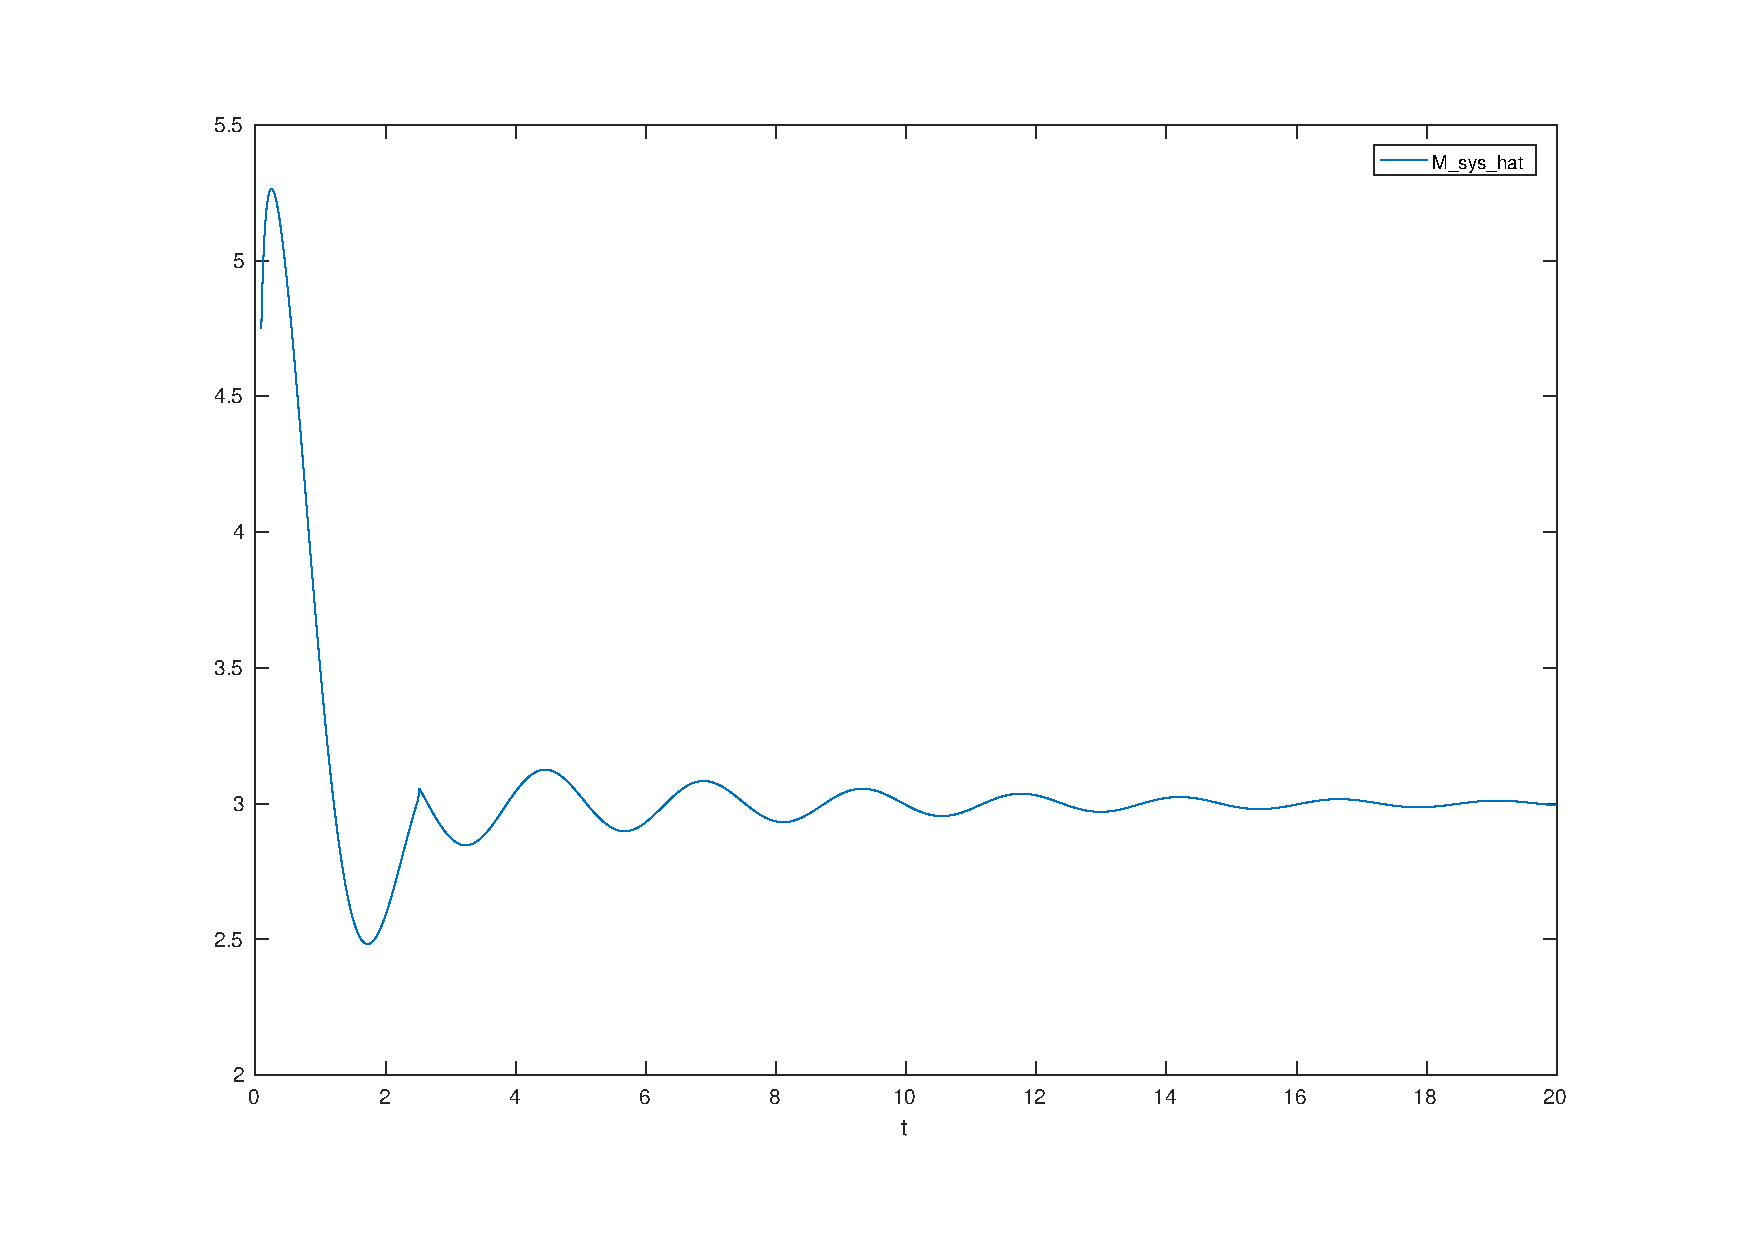
\includegraphics[width=0.99\linewidth]{systemfs500_mass}
	\centering
	\caption{Estymacja masy układu z parametrami $T=0.01$, $k = 20$, $b = 1$, $m = 3$ dla 500 próbek używanych w alogrytmie średniej kroczącej.}
	\label{fig:systemfs500_mass}
\end{figure}


\begin{figure}[H]
	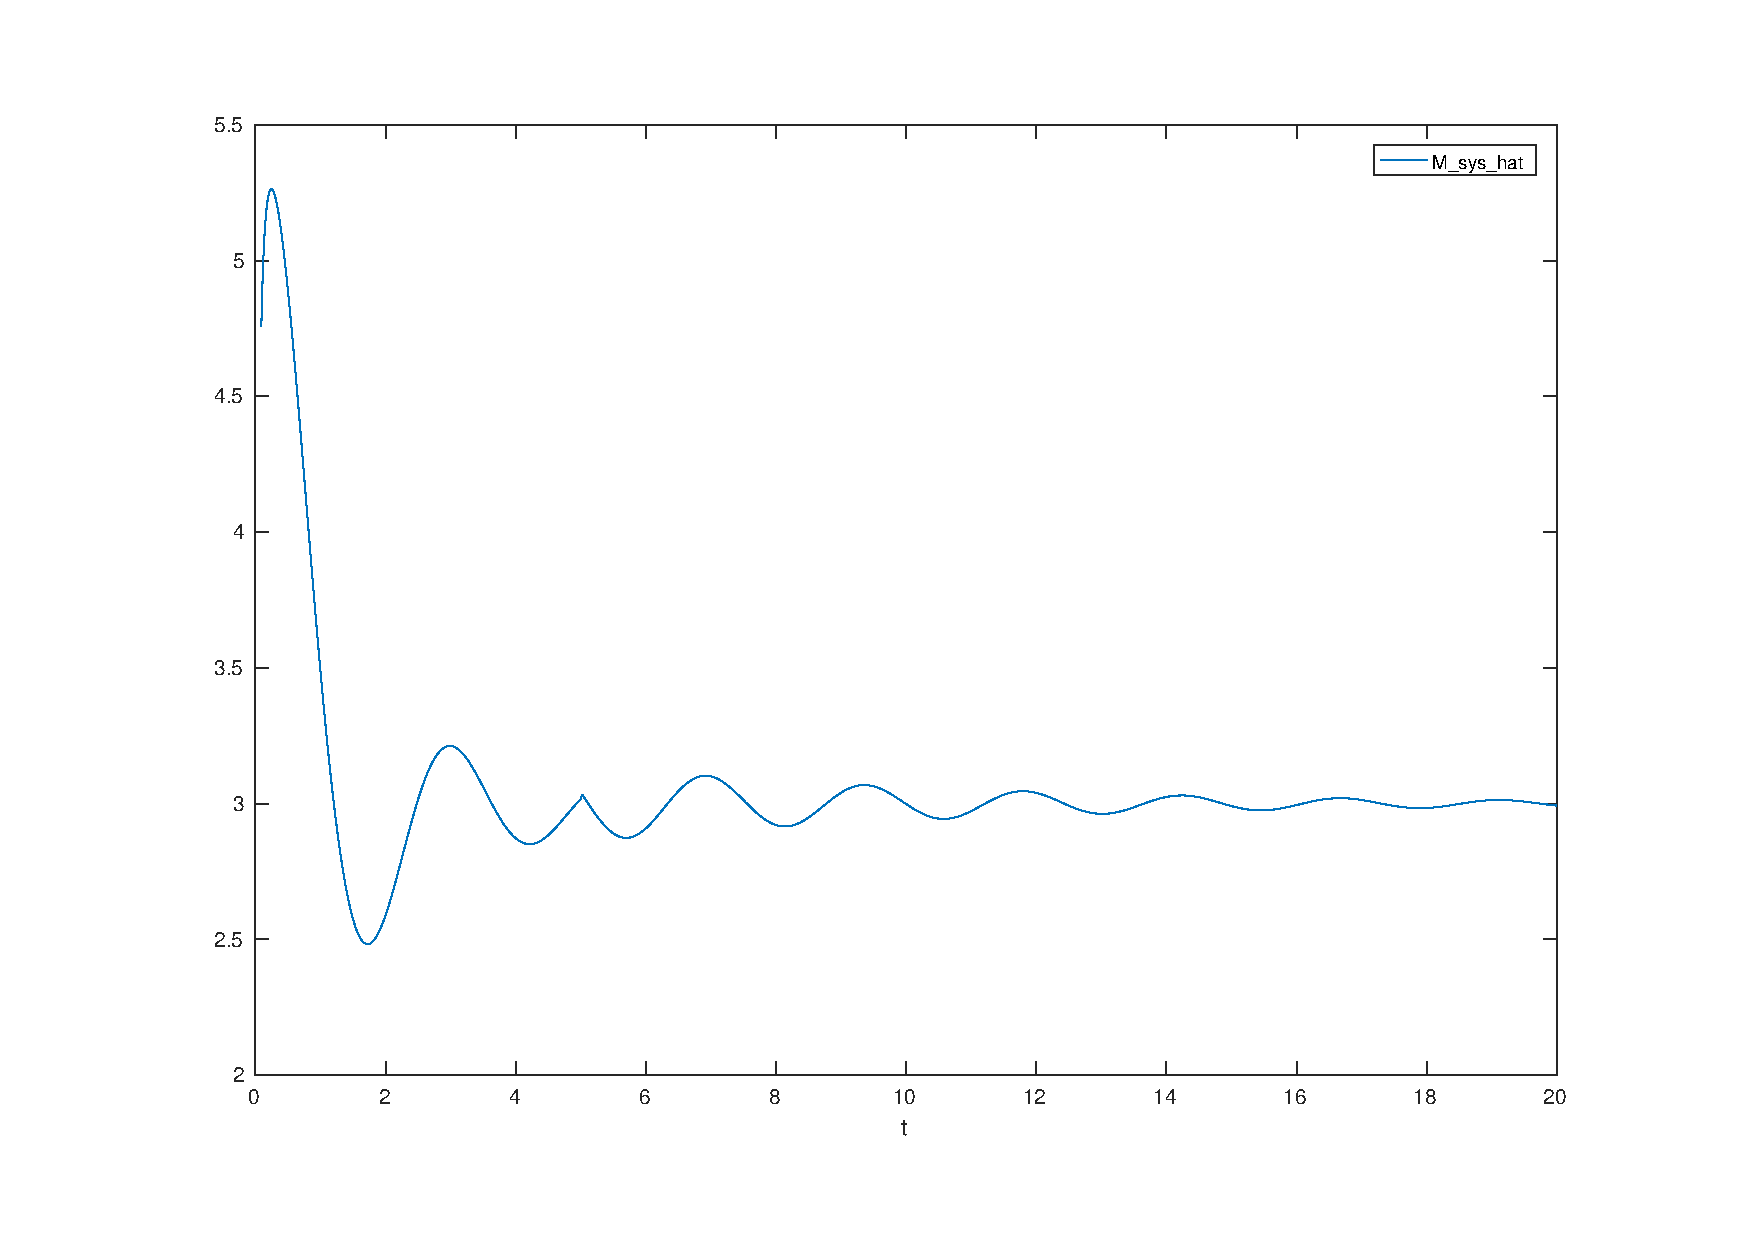
\includegraphics[width=0.99\linewidth]{systemfs1000_mass}
	\centering
	\caption{Estymacja masy układu z parametrami $T=0.01$, $k = 20$, $b = 1$, $m = 3$ dla 1000 próbek używanych w alogrytmie średniej kroczącej. }
	\label{fig:systemfs1000_mass}
\end{figure}



W trakcie symulacji eksperymentowano z różną ilością próbek stosowanych do estymacji (rys. \ref{fig:system4_mass}, \ref{fig:system20_mass}, \ref{fig:system200_mass}). Ostatecznie przyjęto $n = 100$ (rys. \ref{fig:system100_mass}). Szczególnie dla mniejszej ilości próbek używanych do optymalizacji można zauważyć pogorszenie jakości estymacji w momencie gdy przyspieszenie układu jest małe. Dla zwiększonej liczby próbek widać polepszenie jakości estymacji kosztem czasu jej uzyskania. Podczas eksperymentów stwierdzono, że estymacja wykazuje dużą podatność na zakłócenia. Dlatego finalnie zdecydowano się na zastosowanie algorytmu średniej kroczącej w celu odfiltrowania zakłóceń (rys. \ref{fig:filter_mass})

\begin{figure}[H]
	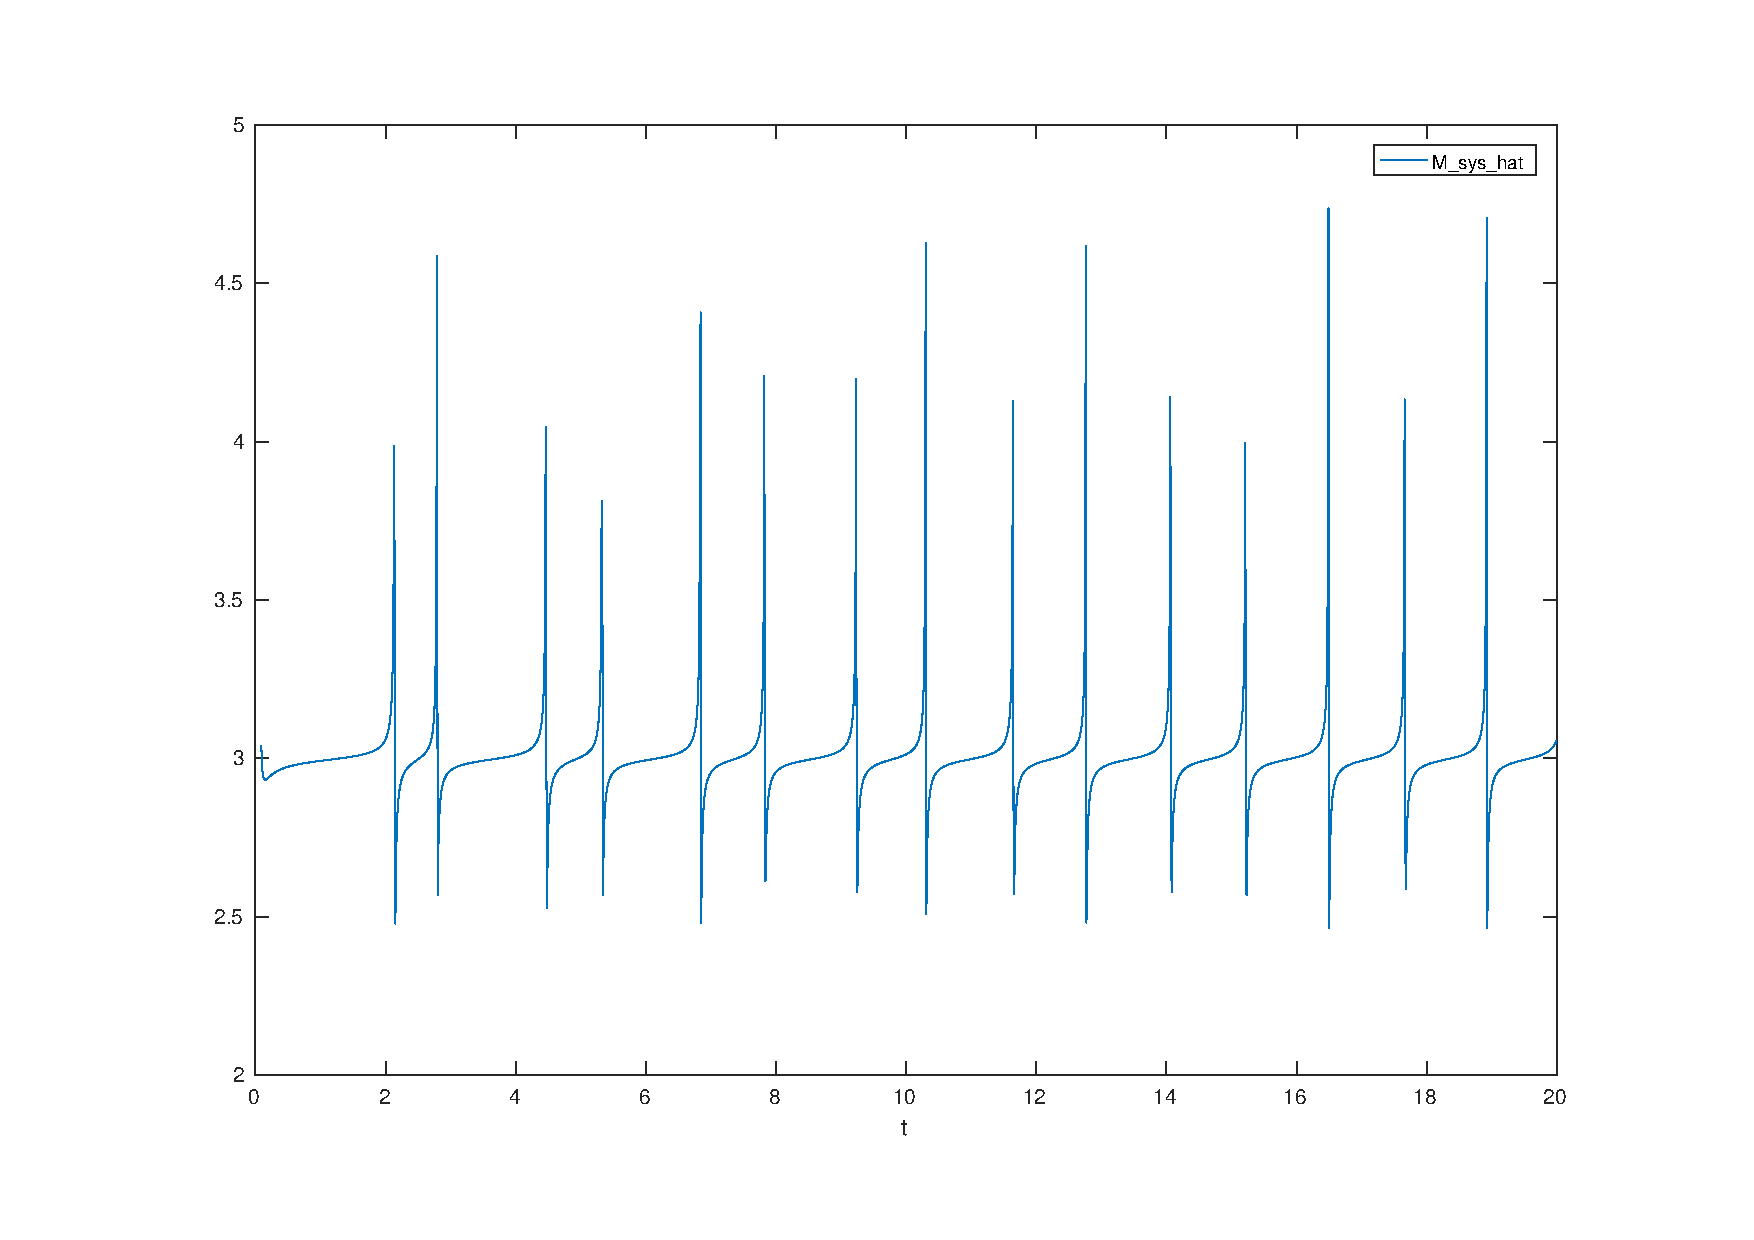
\includegraphics[width=0.99\linewidth]{system4_mass}
	\centering
	\caption{Estymacja masy układu z parametrami $T=0.01$, $k = 20$, $b = 1$, $m = 3$ dla 4 próbek optymalizacji. }
	\label{fig:system4_mass}
\end{figure}

\begin{figure}[H]
	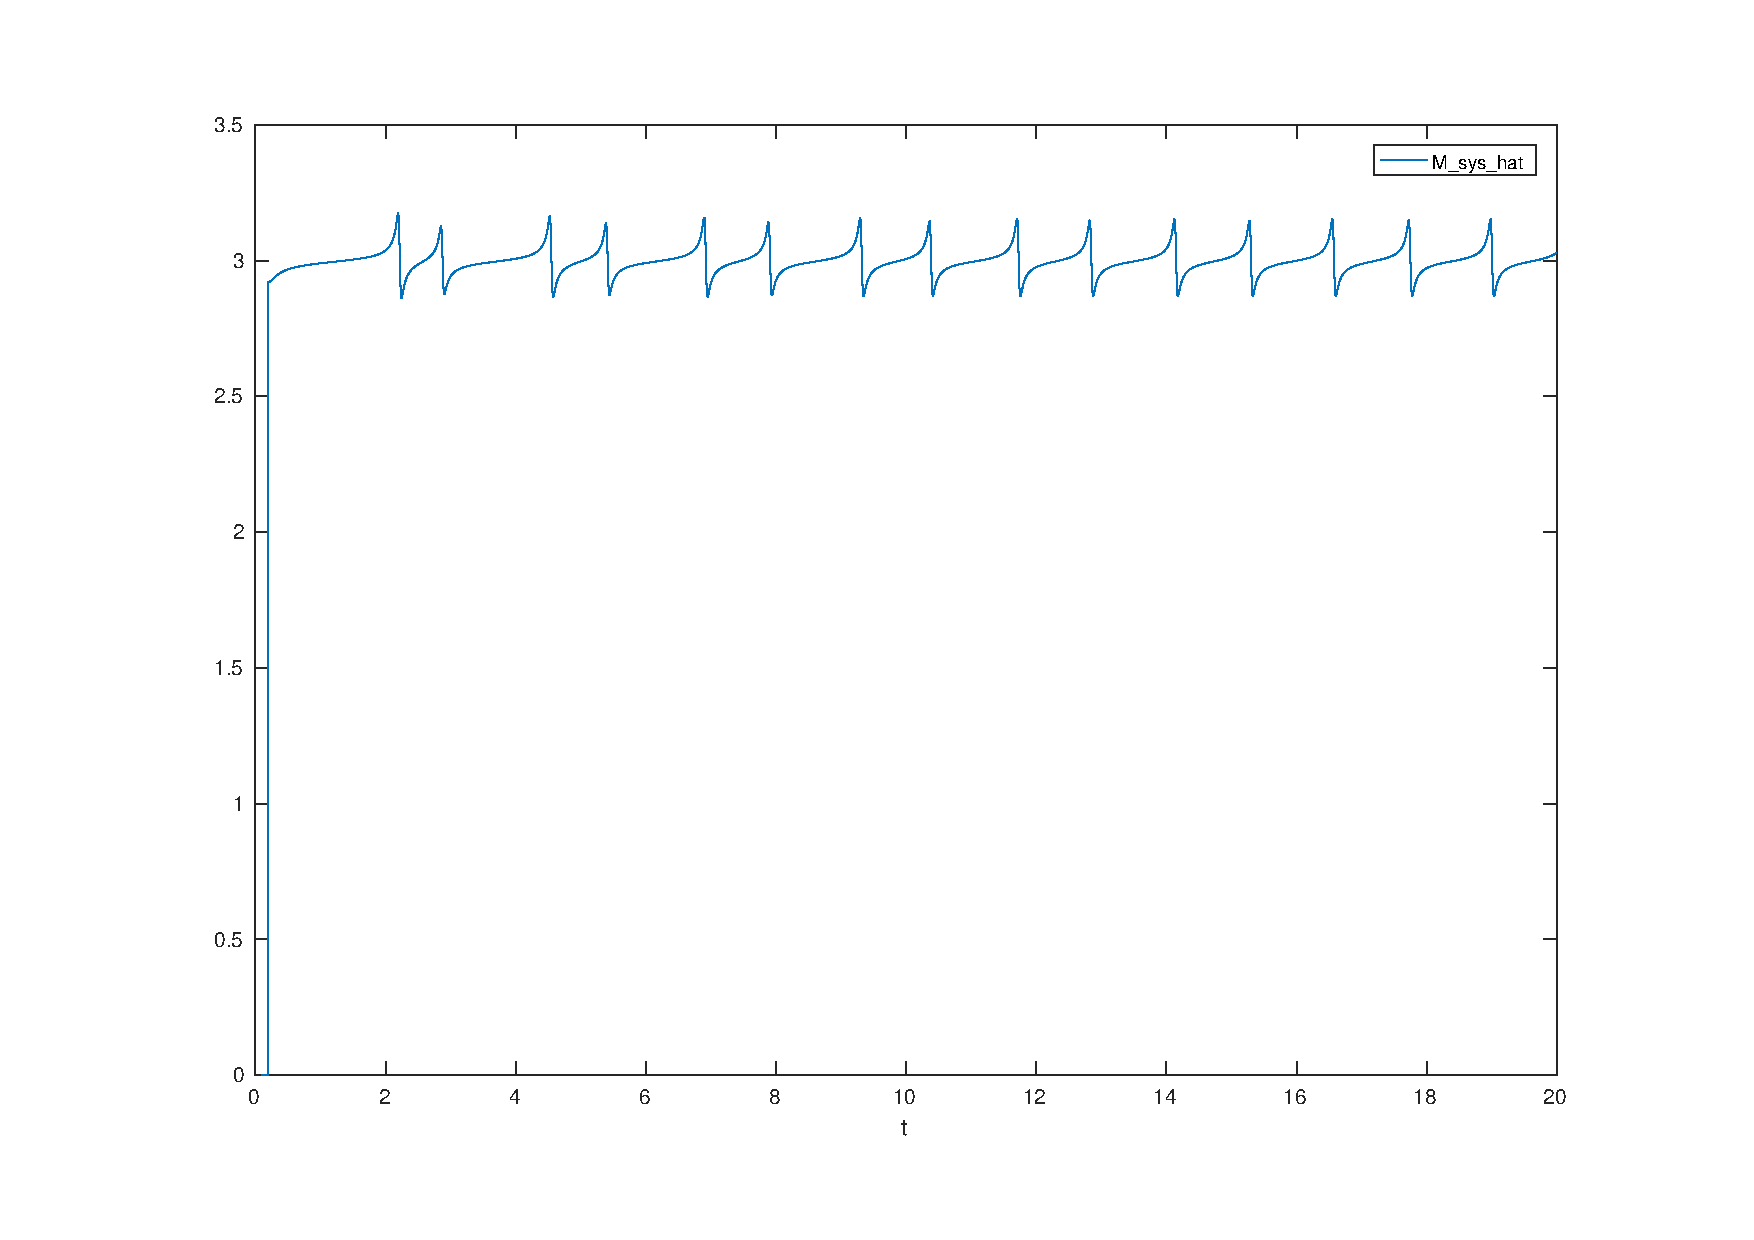
\includegraphics[width=0.99\linewidth]{system20_mass}
	\centering
	\caption{Estymacja masy układu z parametrami $T=0.01$, $k = 20$, $b = 1$, $m = 3$ dla 20 próbek optymalizacji.}
	\label{fig:system20_mass}
\end{figure}

\begin{figure}[H]
	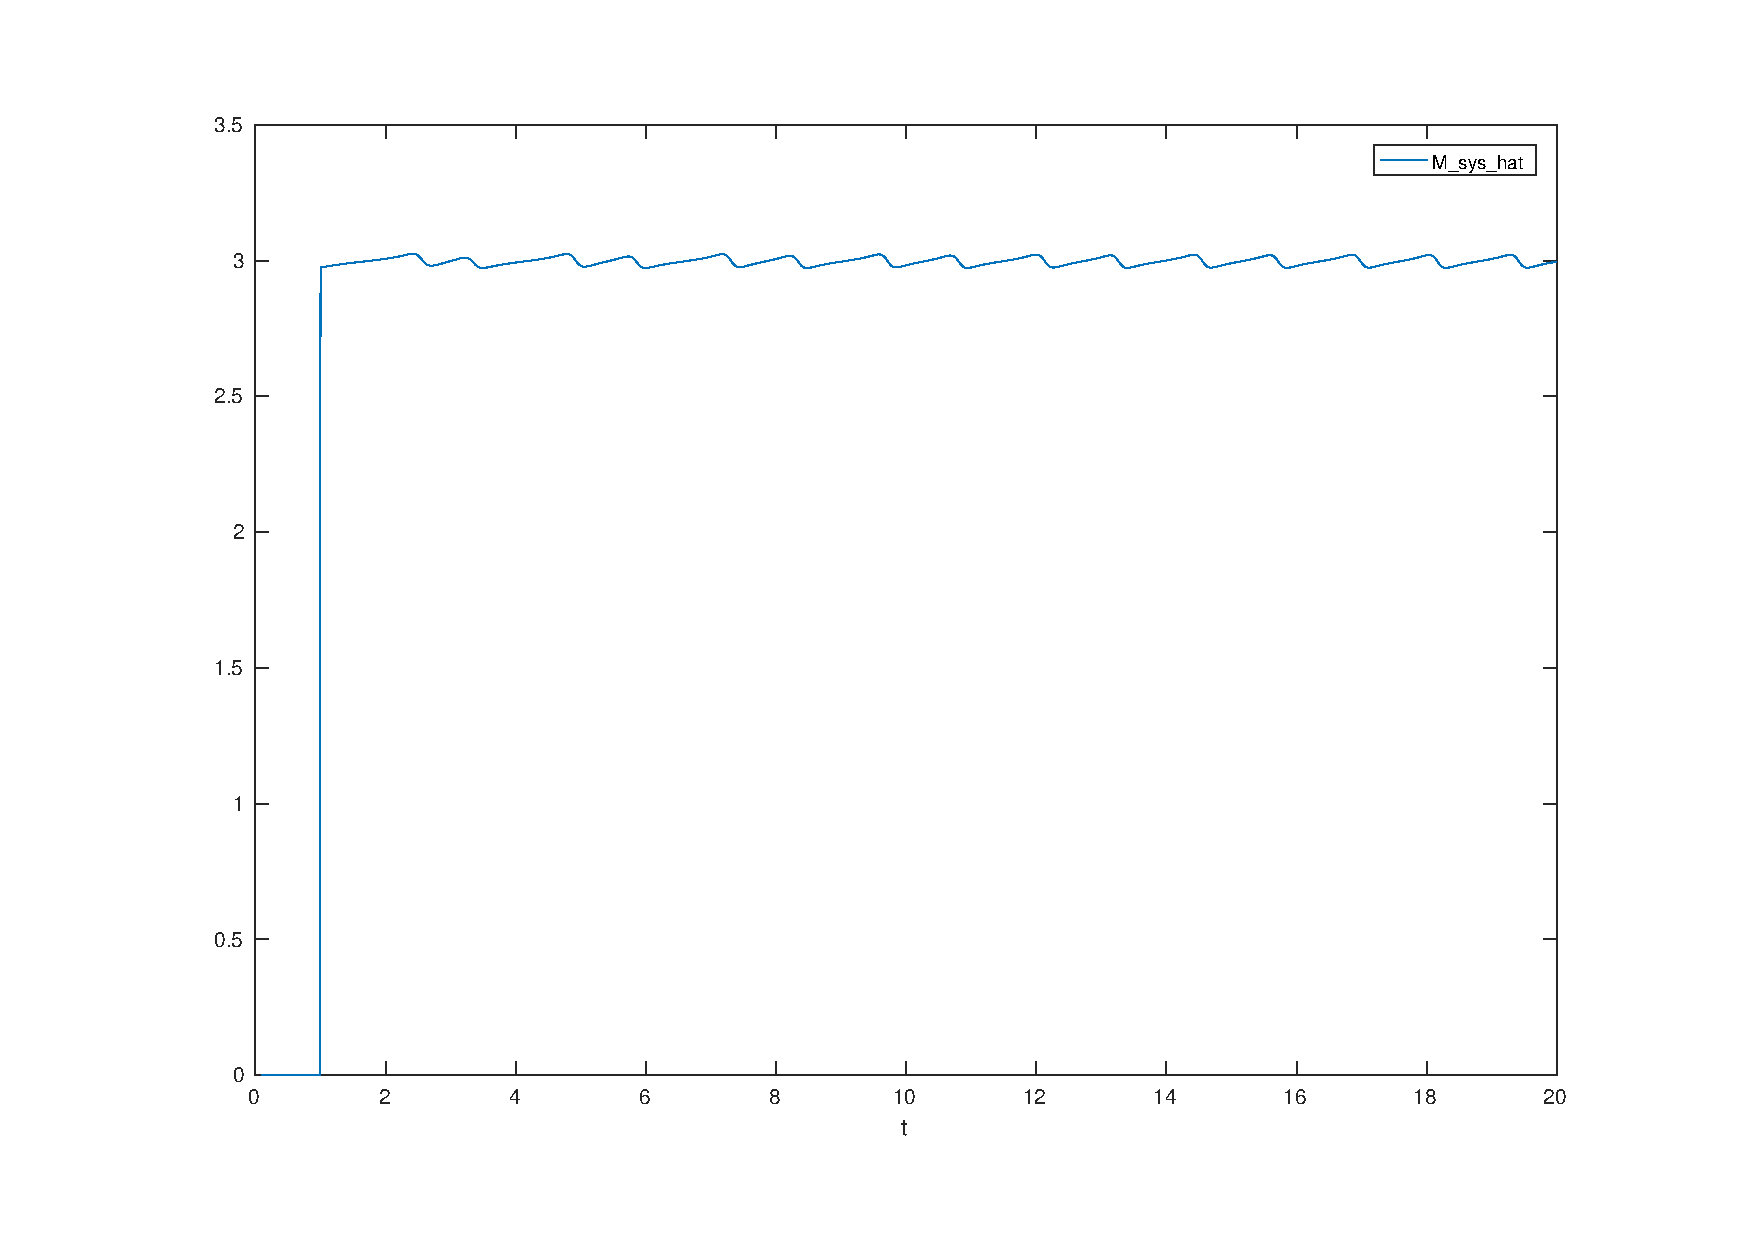
\includegraphics[width=0.99\linewidth]{system100_mass}
	\centering
	\caption{Estymacja masy układu z parametrami $T=0.01$, $k = 20$, $b = 1$, $m = 3$ dla 100 próbek optymalizacji.}
	\label{fig:system100_mass}
\end{figure}

\begin{figure}[H]
	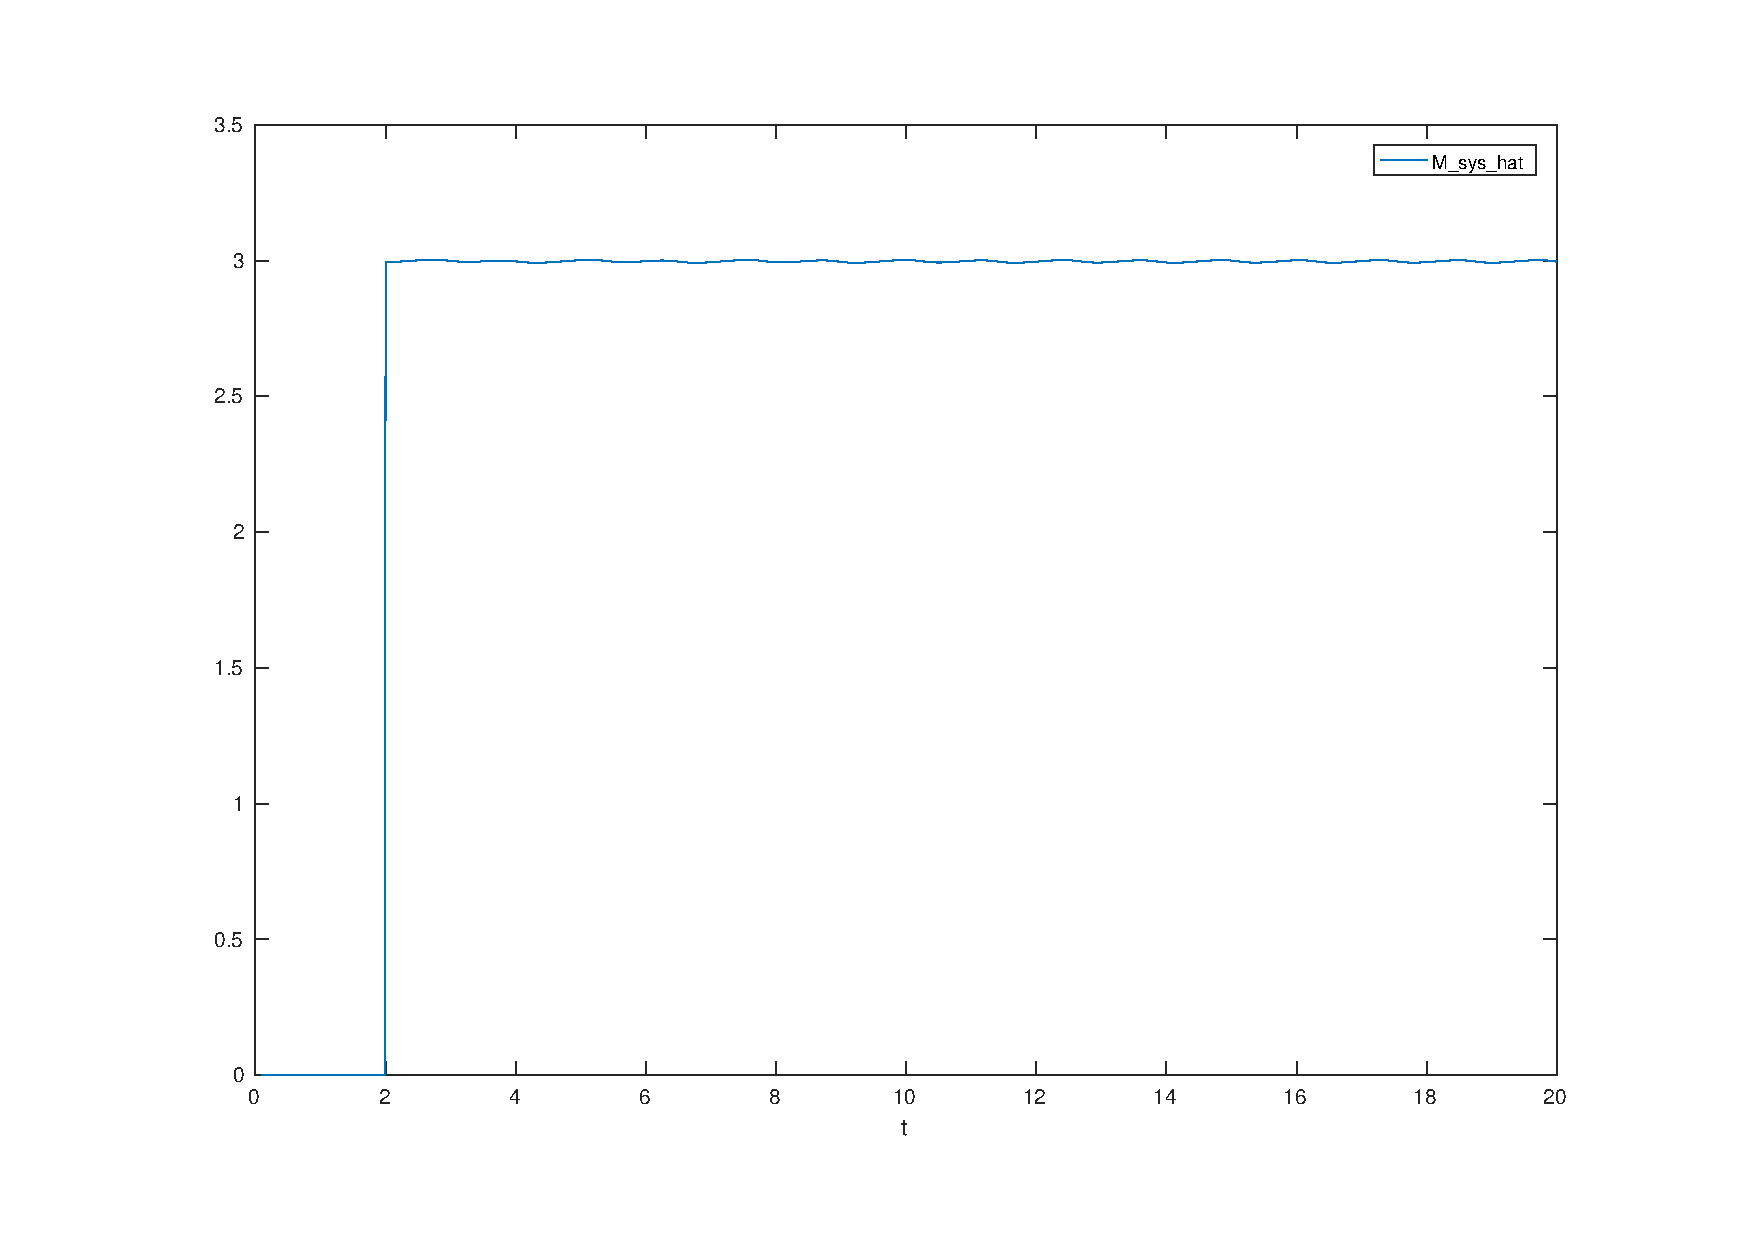
\includegraphics[width=0.99\linewidth]{system200_mass}
	\centering
	\caption{Estymacja masy układu z parametrami $T=0.01$, $k = 20$, $b = 1$, $m = 3$ dla 200 próbek optymalizacji.}
	\label{fig:system200_mass}
\end{figure}

\begin{figure}[H]
	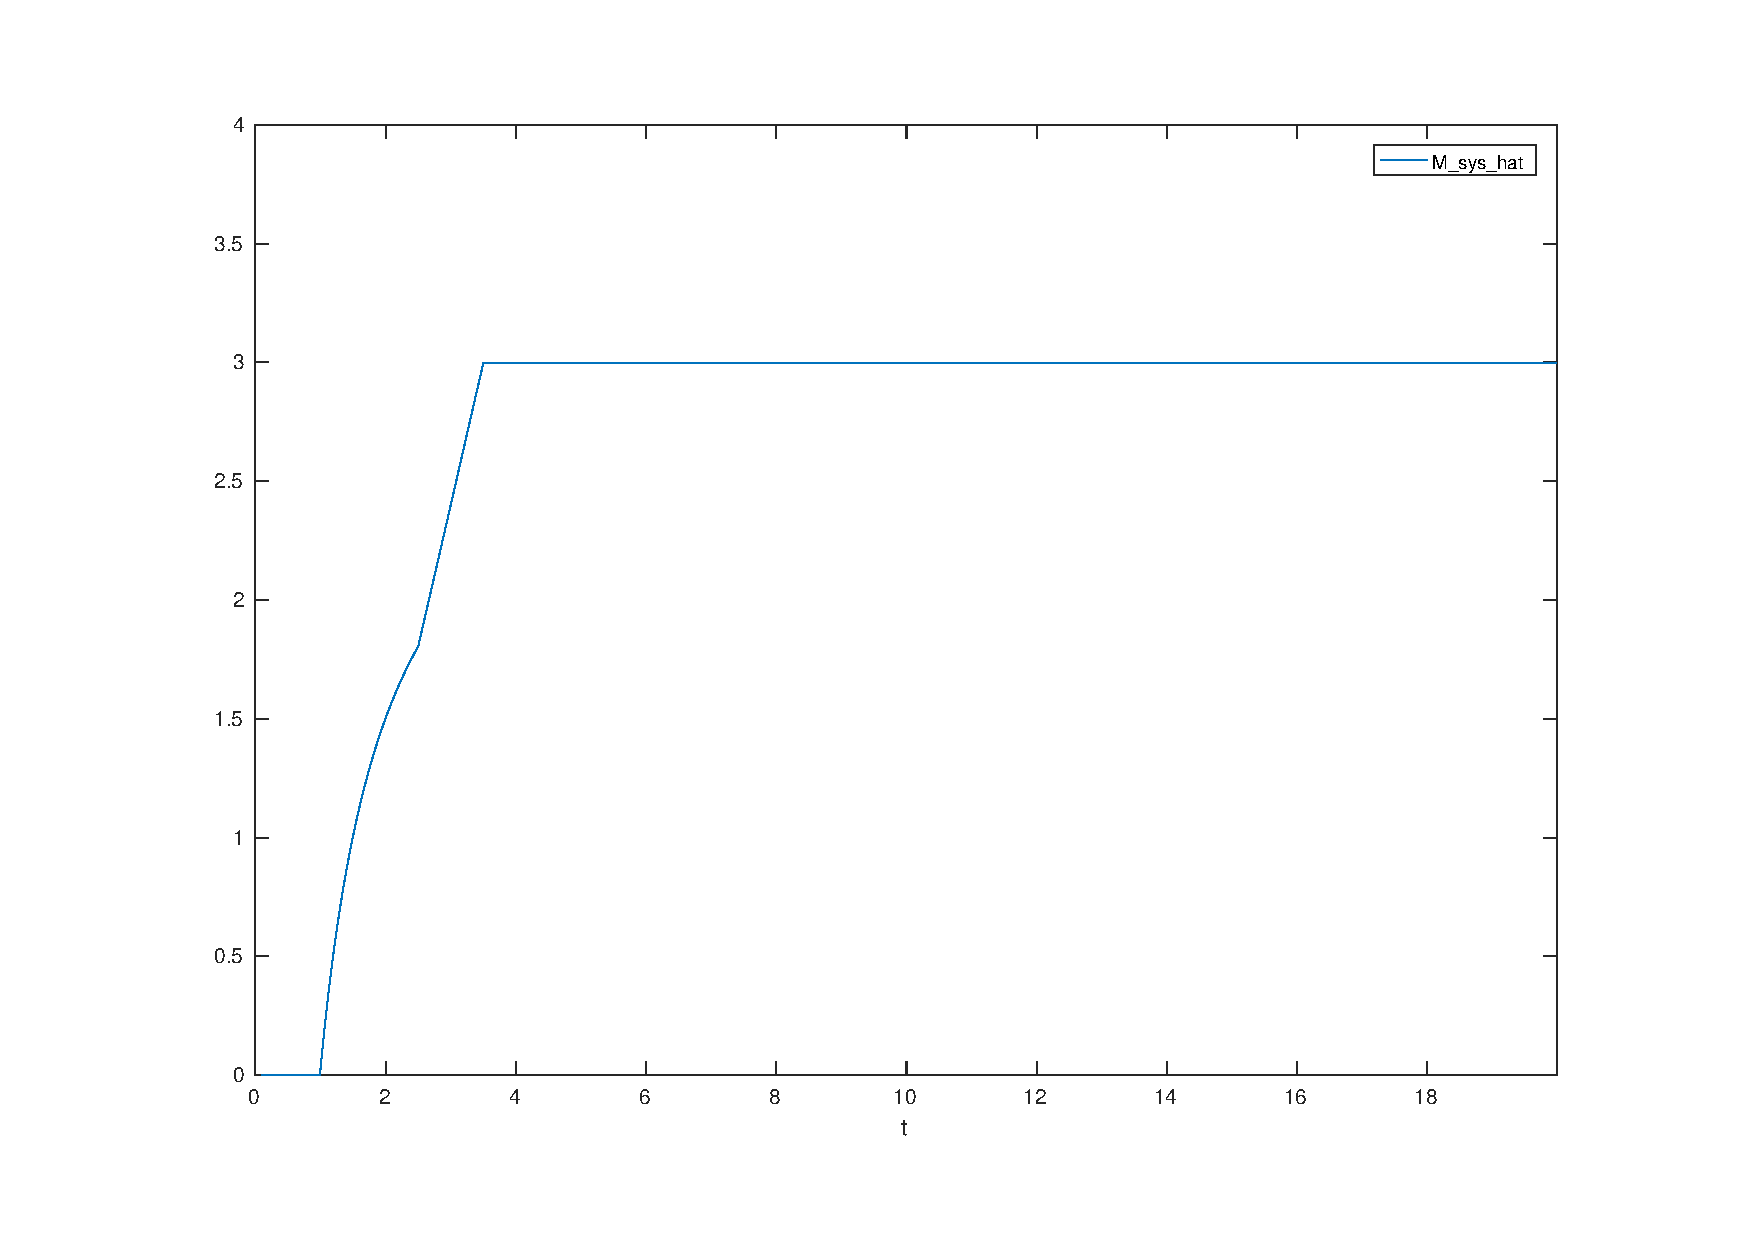
\includegraphics[width=0.99\linewidth]{filter_mass}
	\centering
	\caption{Estymacja masy układu z parametrami $T=0.01$, $k = 20$, $b = 1$, $m = 3$ dla 100 próbek optymalizacji i po zastosowaniu filtru średniej kroczącej.}
	\label{fig:filter_mass}
\end{figure}


\section{Estymacja masy}
Estymacja masy działa na podstawie dwóch modeli. Model opisany w sekcji \ref{fs} działa dobrze gdy układ jest ustabilizowany. Model opisany w sekcji \ref{pos} działa dobrze gdy układ jest w ruchu. W celu poprawnej estymacji w dowolnym momencie pracy układu połączono dane z modeli przy wykorzystaniu logiki rozmytej (rys. \ref{fig:system_mass}). Funkcja przynależności (rys. \ref{fig:system_w}) decyduje o większym udziale modelu czujnika siły w momencie gdy na układ nie działają przyspieszenia.

\begin{figure}[H]
	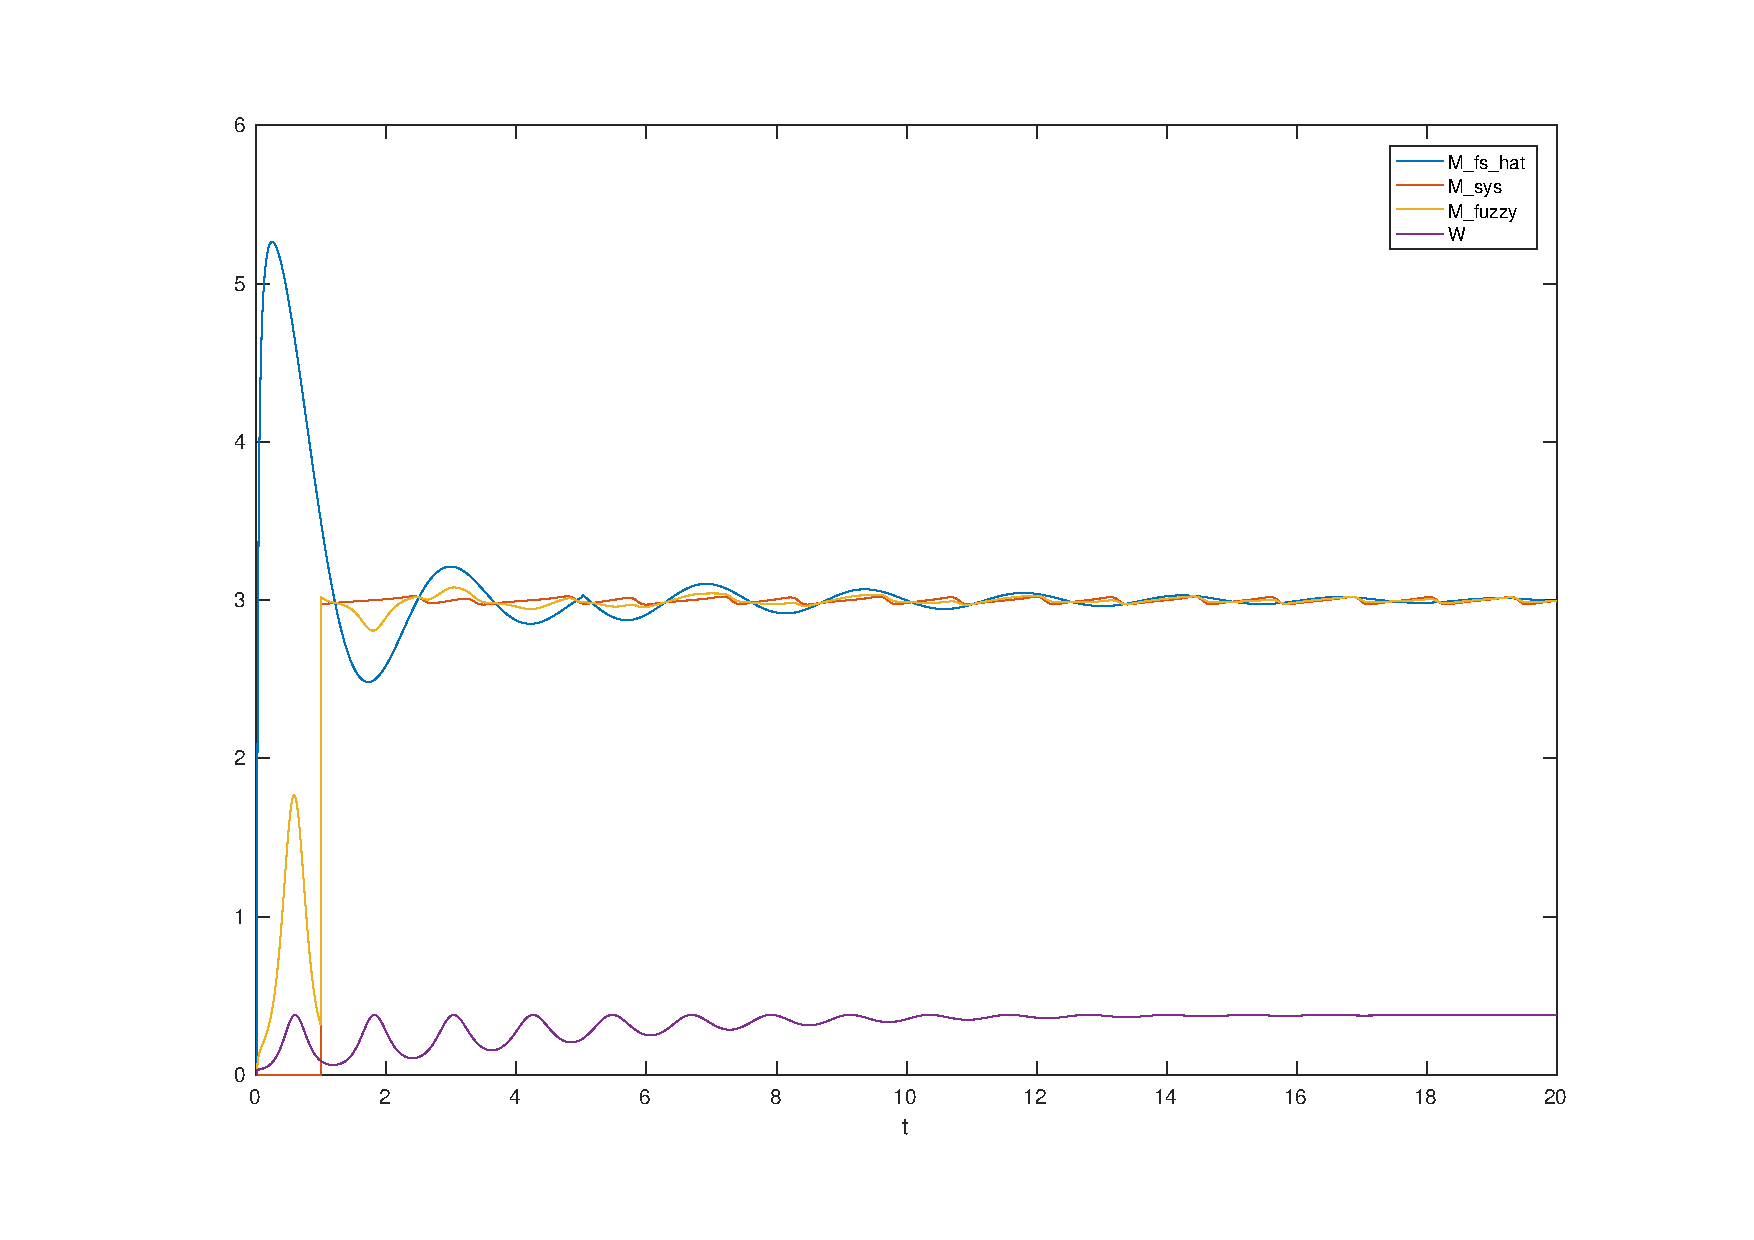
\includegraphics[width=0.99\linewidth]{system_mass}
	\centering
	\caption{Estymacja masy układu z parametrami $T=0.01$, $k = 20$, $b = 1$, $m = 3$. Linią $W$ oznaczono poziom funkcji przynależności modelu }
	\label{fig:system_mass}
\end{figure}

\begin{figure}[H]
	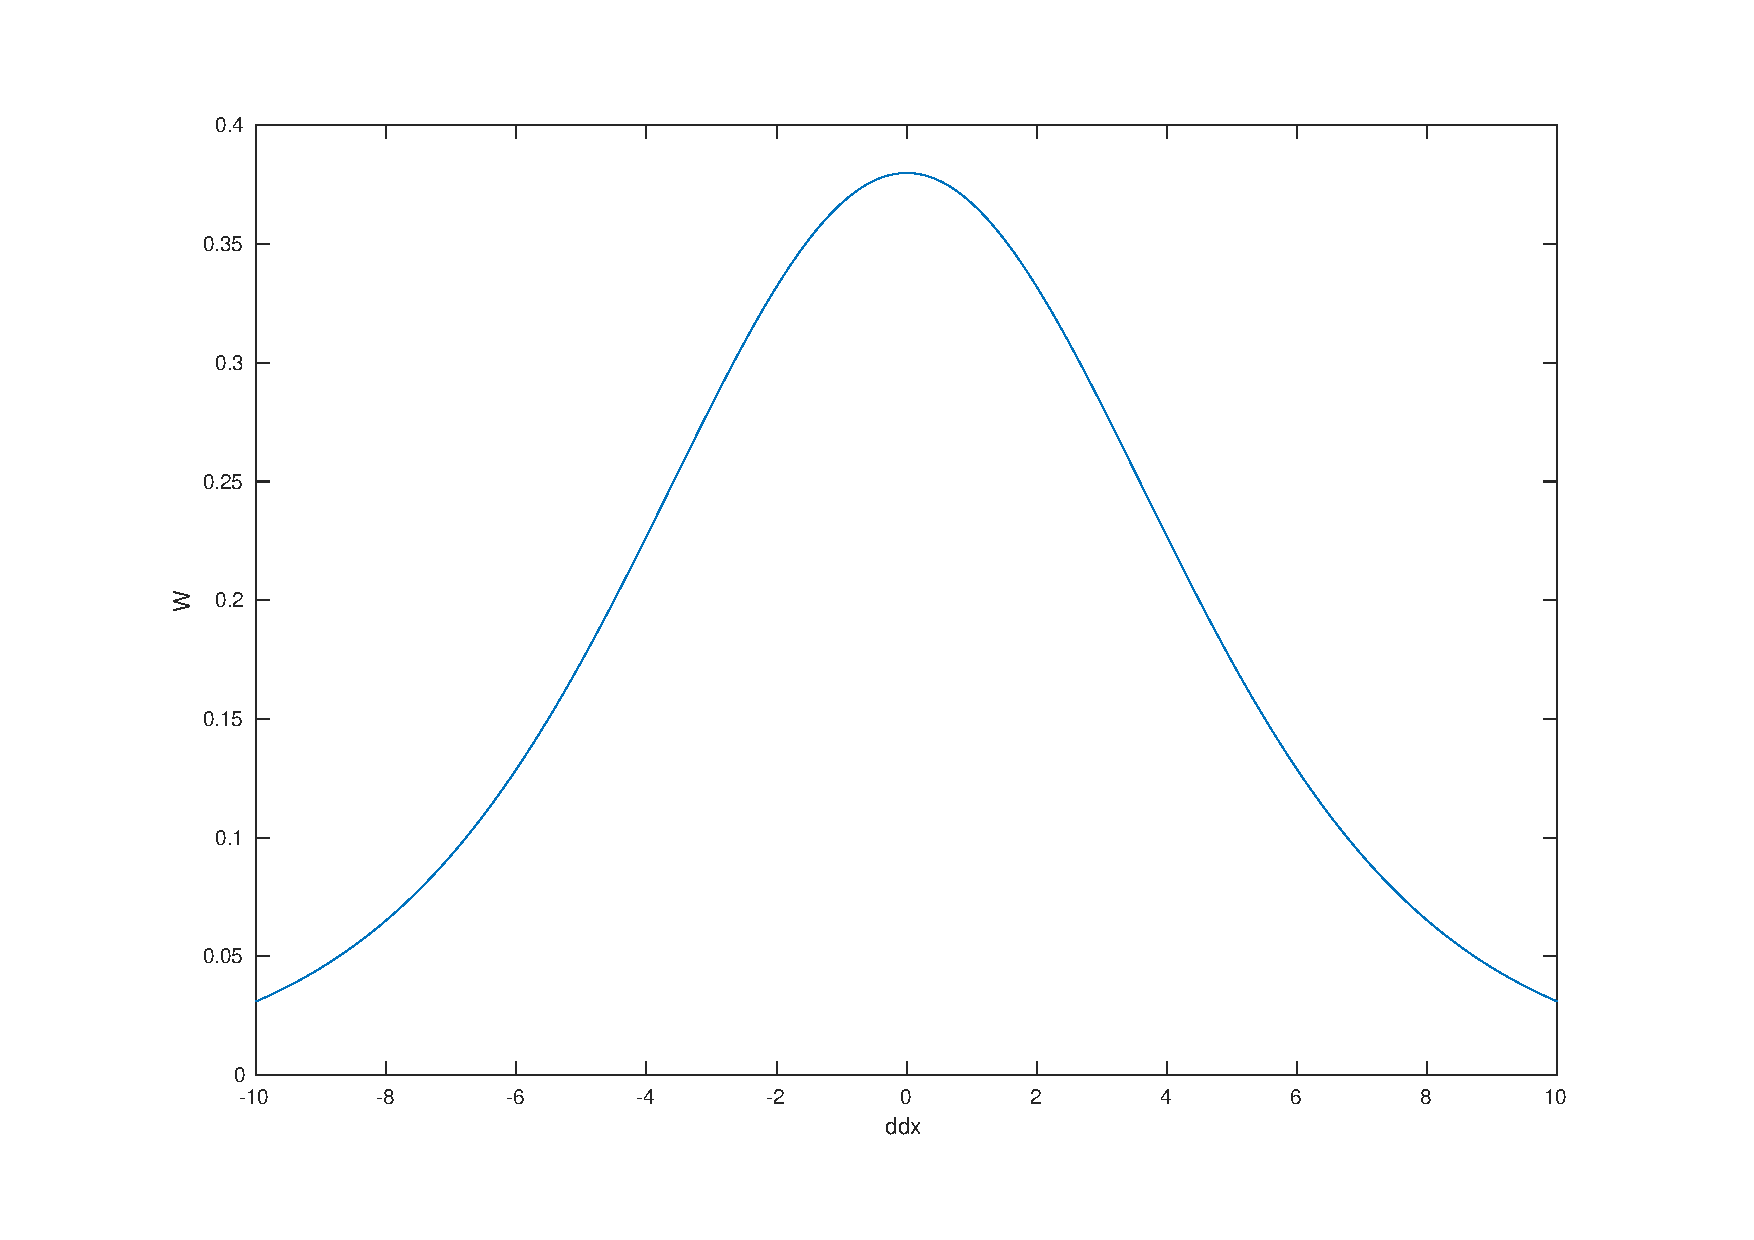
\includegraphics[width=0.99\linewidth]{system_w}
	\centering
	\caption{Sigmoidalna funkcja przynależności postaci $f(\ddot{x}; a, c) = \frac{1}{1+e^{\|\ddot{x}\|-c}}$ z parametrami $a~=~0.4$, $c = 2$.}
	\label{fig:system_w}
\end{figure}





\section{Kompensacja grawitacji}
Kompensacja polega na dodaniu do układu siły która przeciwdziała sile grawitacji masy.
W celu weryfikacji kompensacji siły grawitacji należy zastanowić się jak wyglądać powinny przebiegi układu. Można przyjąć, że układ powinien się zachowywać tak jakby nie była na nim zawieszona żadna masa (rys. \ref{fig:systemwm})
W idealnym przypadku (rys. \ref{fig:system_ideal}) układ zachowuje się jak ten pozbawiony masy. W normalnym przypadku (rys. \ref{fig:system_komp}), pomijając niedokładności, układ ze skompensowaną siłą grawitacji  zachowuje się dość dobrze Niwelowany jest wpływ grawitacji a układ stabilizuje się w porządanej pozycji. Kompensacja załączana jest stopniowo i nie uwzględnia energii układu która powstała przed załączeniem kompensacji. Powoduje to oscylacje widoczne w układzie. O tym jak szybko układ z załączoną kompensacją grawitacji się ustabilizuje decydują wartości zmiennych stanu układu w momencie rozpoczęcia kompensacji.


\begin{figure}[H]
	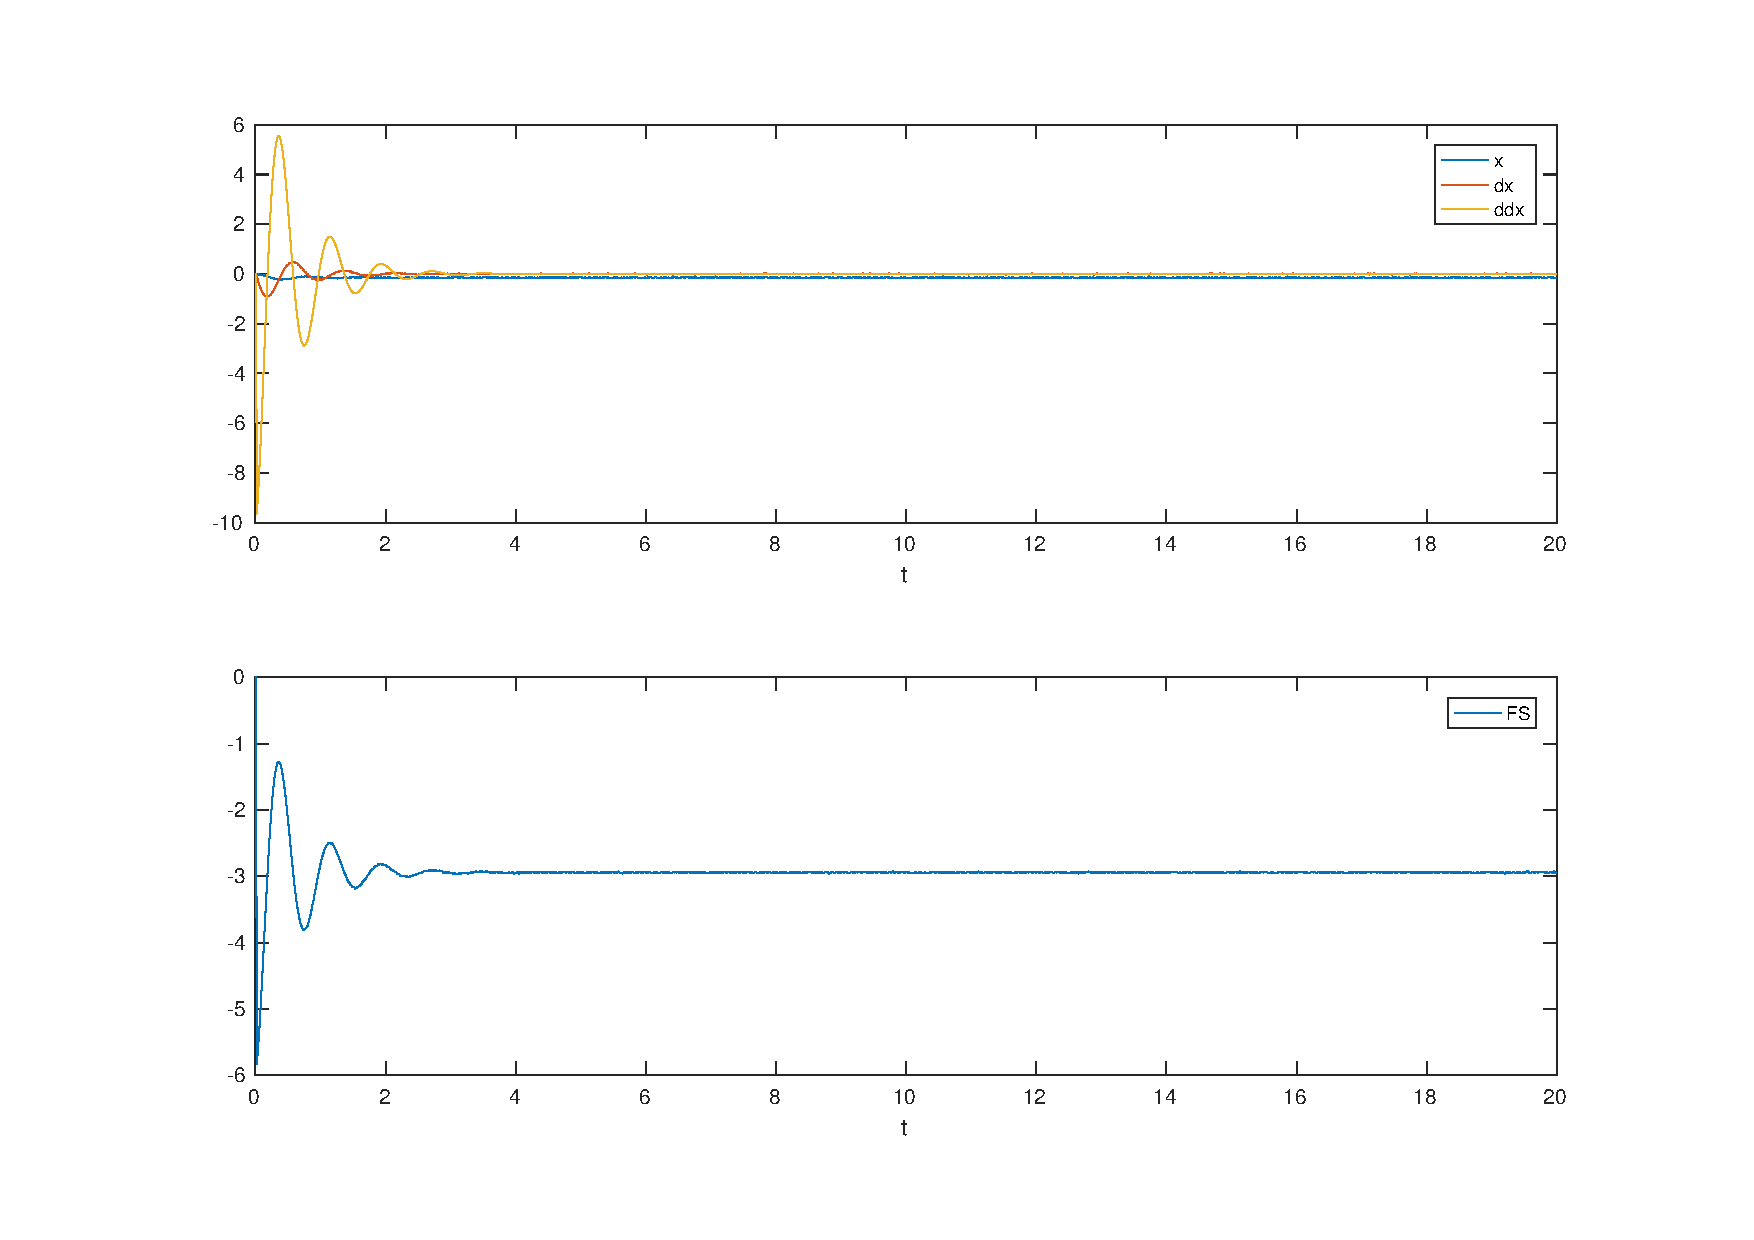
\includegraphics[width=0.99\linewidth]{system_wm_sys}
	\centering
	\caption{Symulacja układu z parametrami $T=0.01$, $k = 20$, $b = 1$, $m = 0.3$. Masa jest 10 razy mniejsza niż początkowego układu.}
	\label{fig:systemwm}
\end{figure}

\begin{figure}[H]
	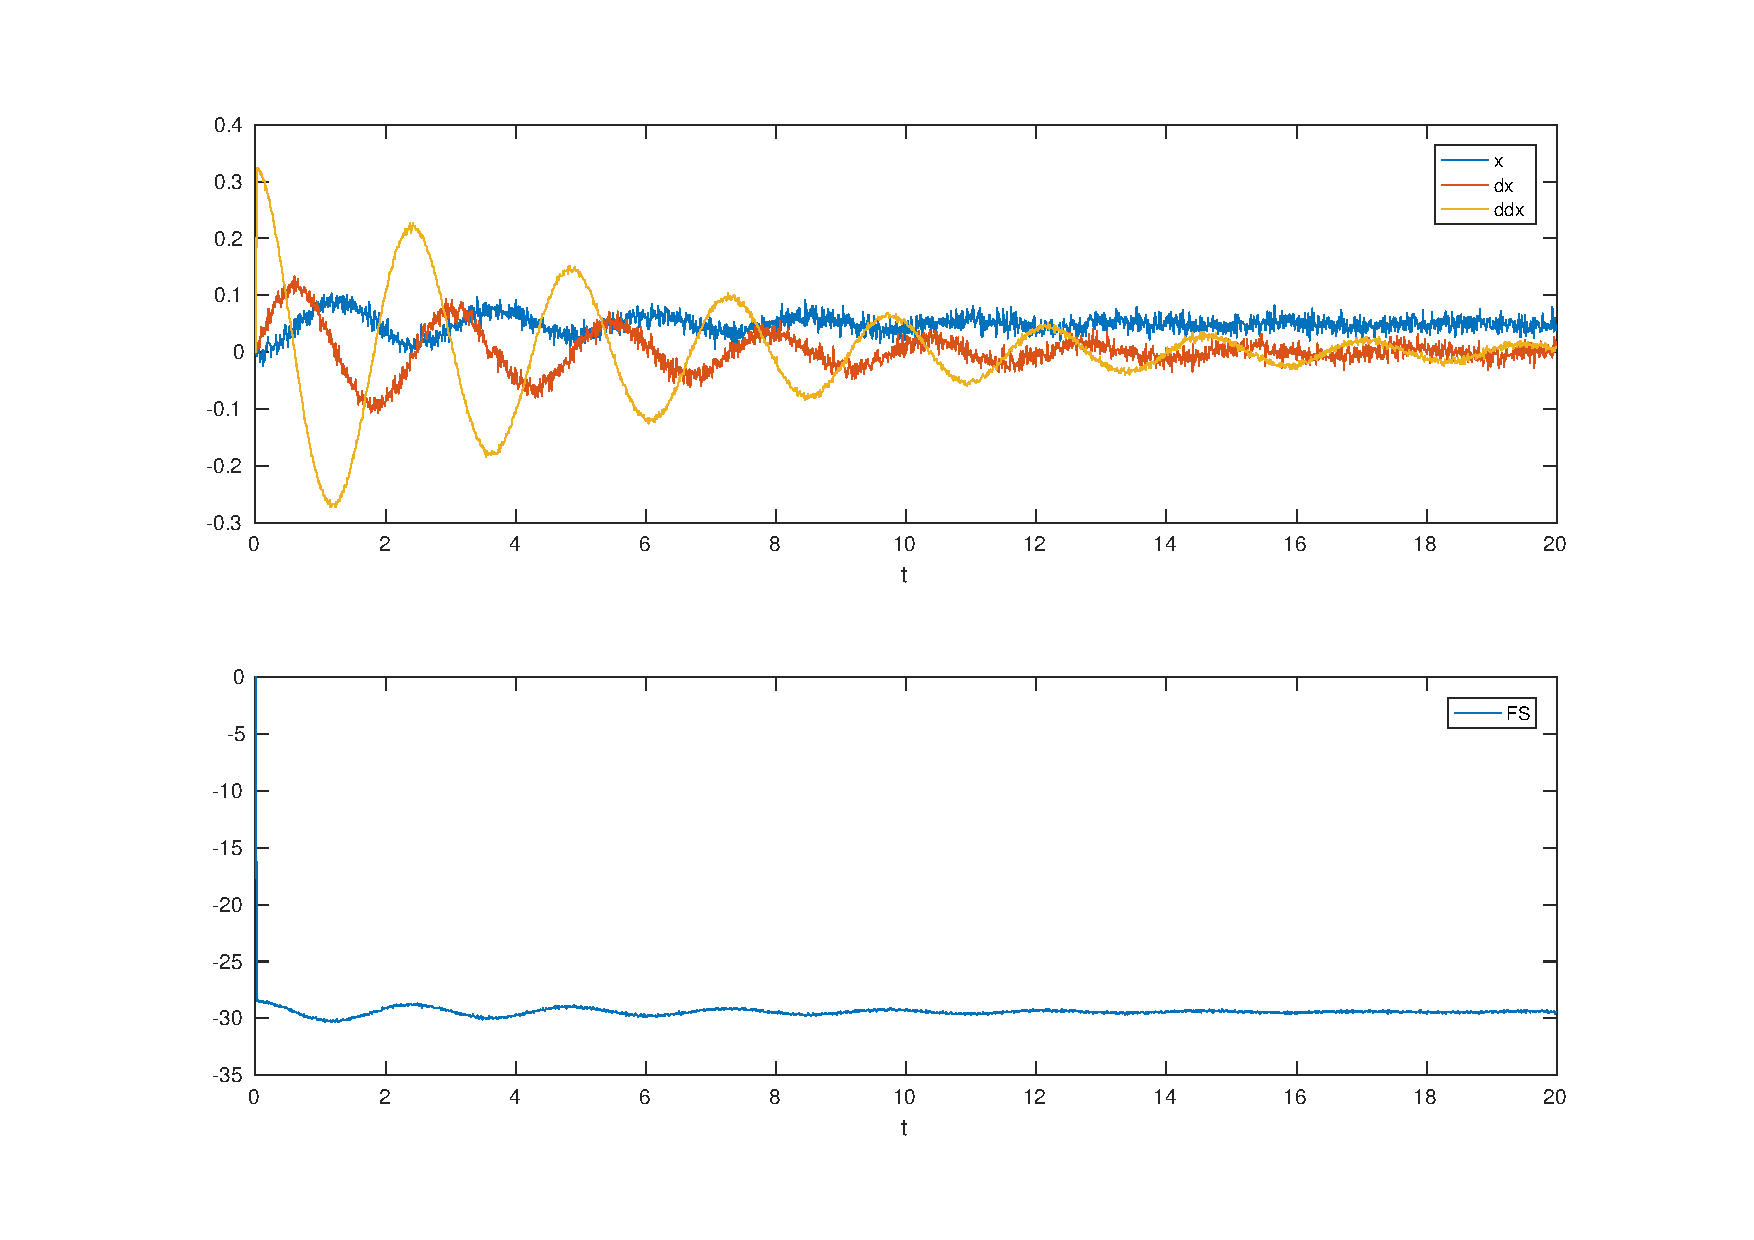
\includegraphics[width=0.99\linewidth]{grav_ideal_sys}
	\centering
	\caption{Symulacja układu z parametrami $T=0.01$, $k = 20$, $b = 1$, $m = 0.3$. Oraz załączoną kompensacją grawitacji.}
	\label{fig:system_ideal}
\end{figure}

\begin{figure}[H]
	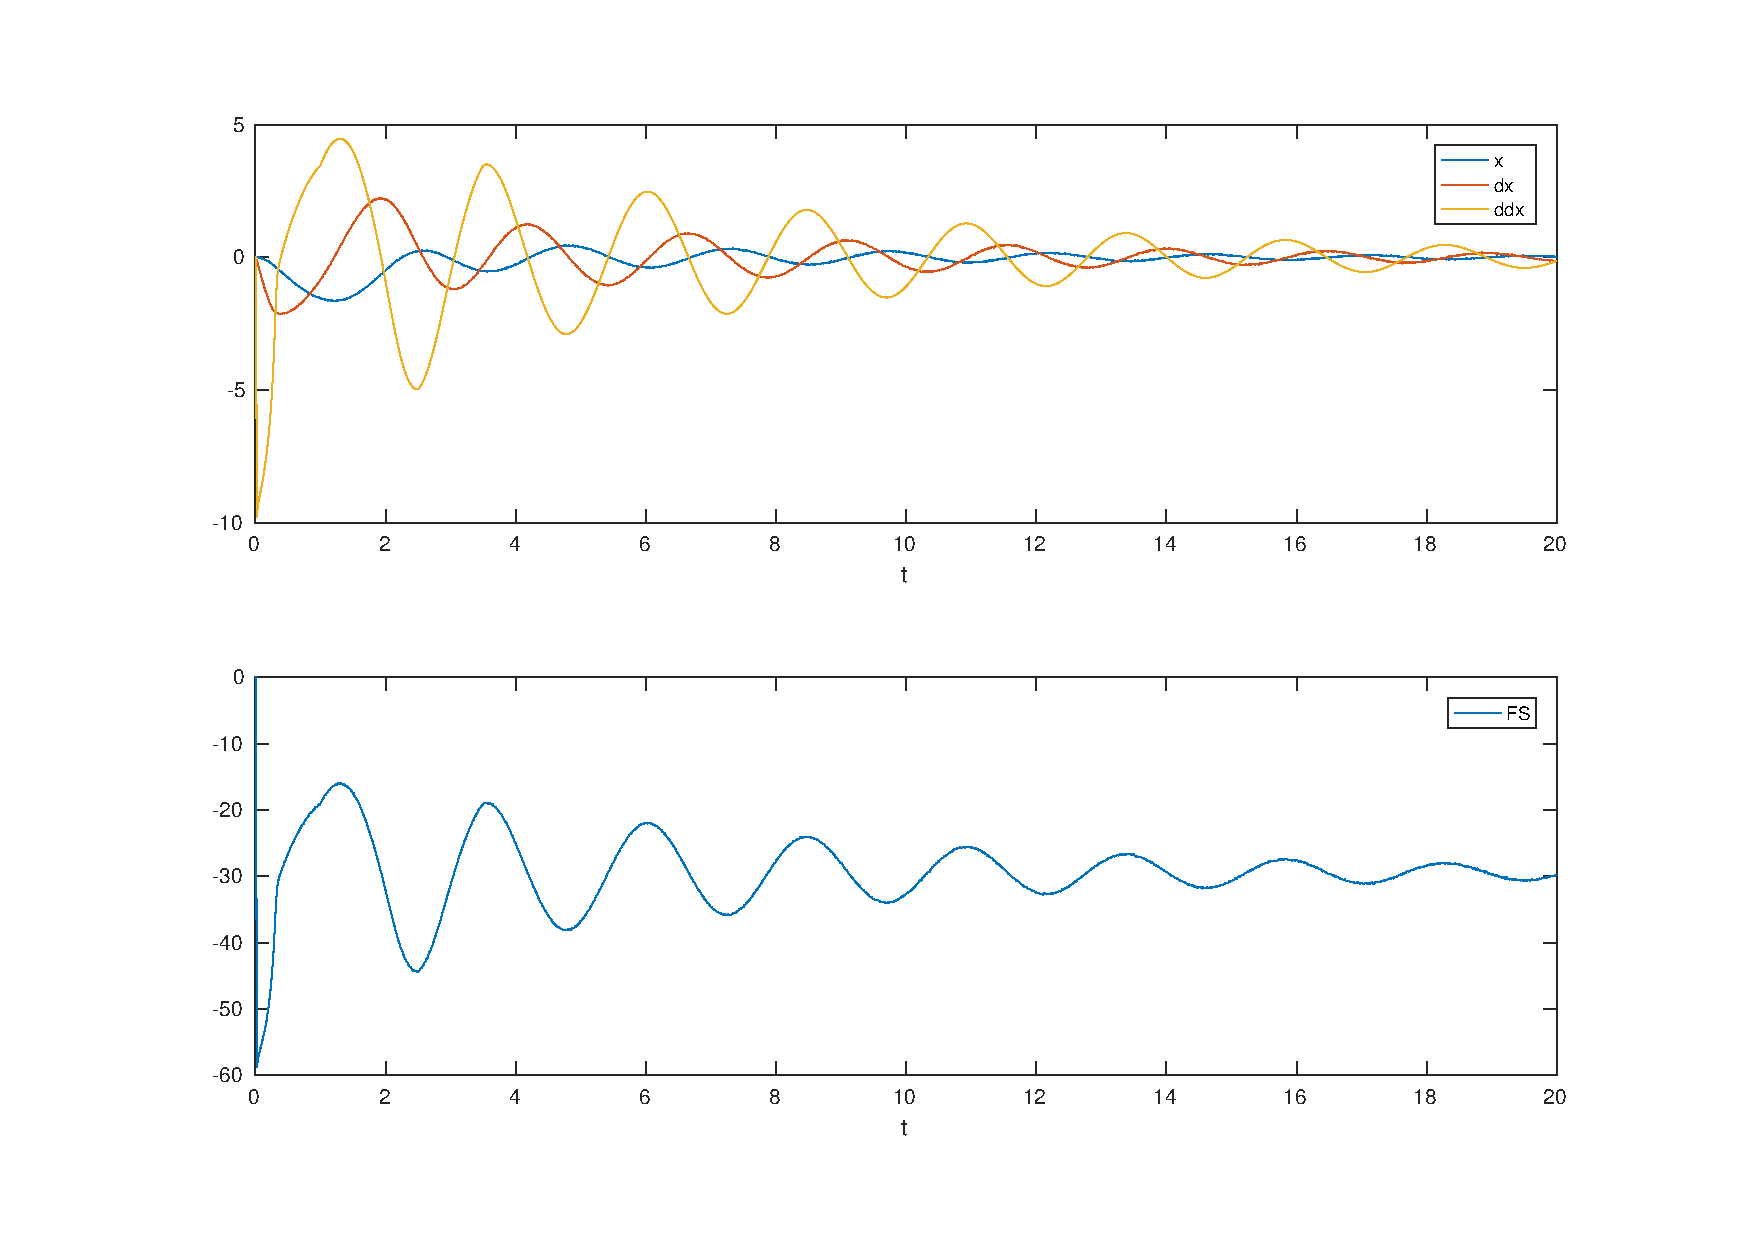
\includegraphics[width=0.99\linewidth]{grav_normal_sys}
	\centering
	\caption{Symulacja układu z parametrami $T=0.01$, $k = 20$, $b = 1$, $m = 0.3$. Oraz załączoną kompensacją grawitacji.}
	\label{fig:system_komp}
\end{figure}

\end{document}